%\newpage
%\begin{tikzpicture}[remember picture, overlay]
%	\node [inner sep=0pt, minimum width=\paperwidth, minimum height=\paperheight,opacity=1,color=Apricot] at (current page.center) {
\includegraphics[width=\paperwidth,height=\paperheight,angle=0]{paper18}};
%
%\end{tikzpicture}
%CUANDO ME VEN, A PESAR DE MI PEQUEÑO TAMAÑO, PUEDEN PENSAR QUE SOY UNA PANTERA NEGRA. S


\iffalse
\newpage
\begin{tikzpicture}[remember picture, overlay]
	\node [inner sep=0pt, minimum width=\paperwidth, minimum height=\paperheight,opacity=.3,color=ForestGreen,fill=ForestGreen] at (current page.center){};
\end{tikzpicture}
\begin{wrapfigure} [7]{l}{.2\textwidth}\vspace{-1.2cm}\hspace{-1.5cm}
	\begin{tikzpicture}
		\node[xscale=-1,yshift=2cm] () {
\includegraphics[width=.25\textwidth]{gato_azul.png}};
	\end{tikzpicture}
	
	\end{wrapfigure}	
ANOCHE SOÑE CON UN GATO AZUL. NUNCA HABÍA VISTO UNO DE ESE COLOR, TAL VEZ CUANDO MIRÉ LA PELÍCULA DE ALICIA EN EL PAÍS DE LAS MARAVILLAS, AQUEL GATO SONRIENTE DE CHESHIRE. PERO NO, EL MÍO NO TENÌA UNA SONRISA DE DIENTES INTERMINABLES, NI JUGABA CON MI CREDULIDAD DESAPARECIENDO Y GIRANDO COMO UN TROMPO. MI GATO AZUL ERA COMO UN PEQUEÑO FANTASMA SERVICIAL QUE PODÍA AYUDARME CON MIS DIBUJOS.

PARA ELLO TENÍA ABIERTOS BIEN GRANDES LOS OJOS, PUES PARA ILUSTRAR BIEN HAY QUE SABER PRIMERO MIRAR. ASÍ COMO PARA HABLAR LO HACEMOS DESPUÉS DE ESCUCHAR Y ESCRIBIR, LUEGO DE LEER. 

MI AMIGO PORTABA UN PLUMÍN SINGULAR.
\newpage
\begin{tikzpicture}[remember picture, overlay]
	\node [inner sep=0pt, minimum width=\paperwidth, minimum height=\paperheight,opacity=.4,color=Apricot] at (current page.center) {
\includegraphics[width=\paperwidth,height=\paperheight,angle=0]{paper27}};
\end{tikzpicture}

CUANDO TRAZÓ CON SU PLUMÍN LA FORMA QUE PUEDEN VER, LO PRIMERO QUE PENSÉ ES QUE IBA A SER UN AUTORETRATO QUE COMENZABA CON SU COLA. LUEGO PENSÉ EXTRAÑADO EN LAS PROPORCIONES Y ME FIGURÉ QUE SE TRATARÍA DE UNA OLA, ASÍ COMO SE LUCEN JUSTO ANTES DE ROMPER EN LA PLAYA.

\begin{wrapfigure} [9]{l}{.45\textwidth}\vspace{-1.2cm}%\hspace{-1.5cm}
	\begin{tikzpicture}
		\node[xscale=1,yshift=0cm] () {
\includegraphics[width=.45\textwidth]{remolino1.png}};
	\end{tikzpicture}
\end{wrapfigure}

LUEGO RECORDÉ LO QUE HABÍA LEÍDO EN EL PRINCIPITO, QUE NADA NECESARIAMENTE ES LO QUE PARECE A LA PRIMERA IMPRESIÓN Y QUE UN SOMBRERO PUEDE EN REALIDAD SER UN ELEFANTE TRAGADO POR UNA GIGANTESCA BOA.
\newpage
\begin{tikzpicture}[remember picture, overlay]
	\node [inner sep=0pt, minimum width=\paperwidth, minimum height=\paperheight,opacity=.3,color=Apricot] at (current page.center) {
\includegraphics[width=\paperwidth,height=\paperheight,angle=0]{paper27}};
\end{tikzpicture}
ASÍ QUE REFLEXIONANDO BIEN, LA PINTURA PUEDE ACOMODARSE COMO UN REMOLINO, GIRANDO COMO UNA ESPIRAL. Y COMO ESTA, HAY FORMAS QUE SE PRESENTAN A TODA ESCALA, DESDE LAS DISTANCIAS ASTRONÓMICAS DE LA GALAXIA, HASTA LAS PEQUEÑAS CADENAS EN LOS NÚCLEOS DE LAS CÉLULAS.

\begin{wrapfigure}[8]{r}{.35\textwidth}
	\vspace{-1.8cm}
	\hspace{-2.6cm}
		\begin{tikzpicture}
			\node[xscale=1.,yshift=0cm] () {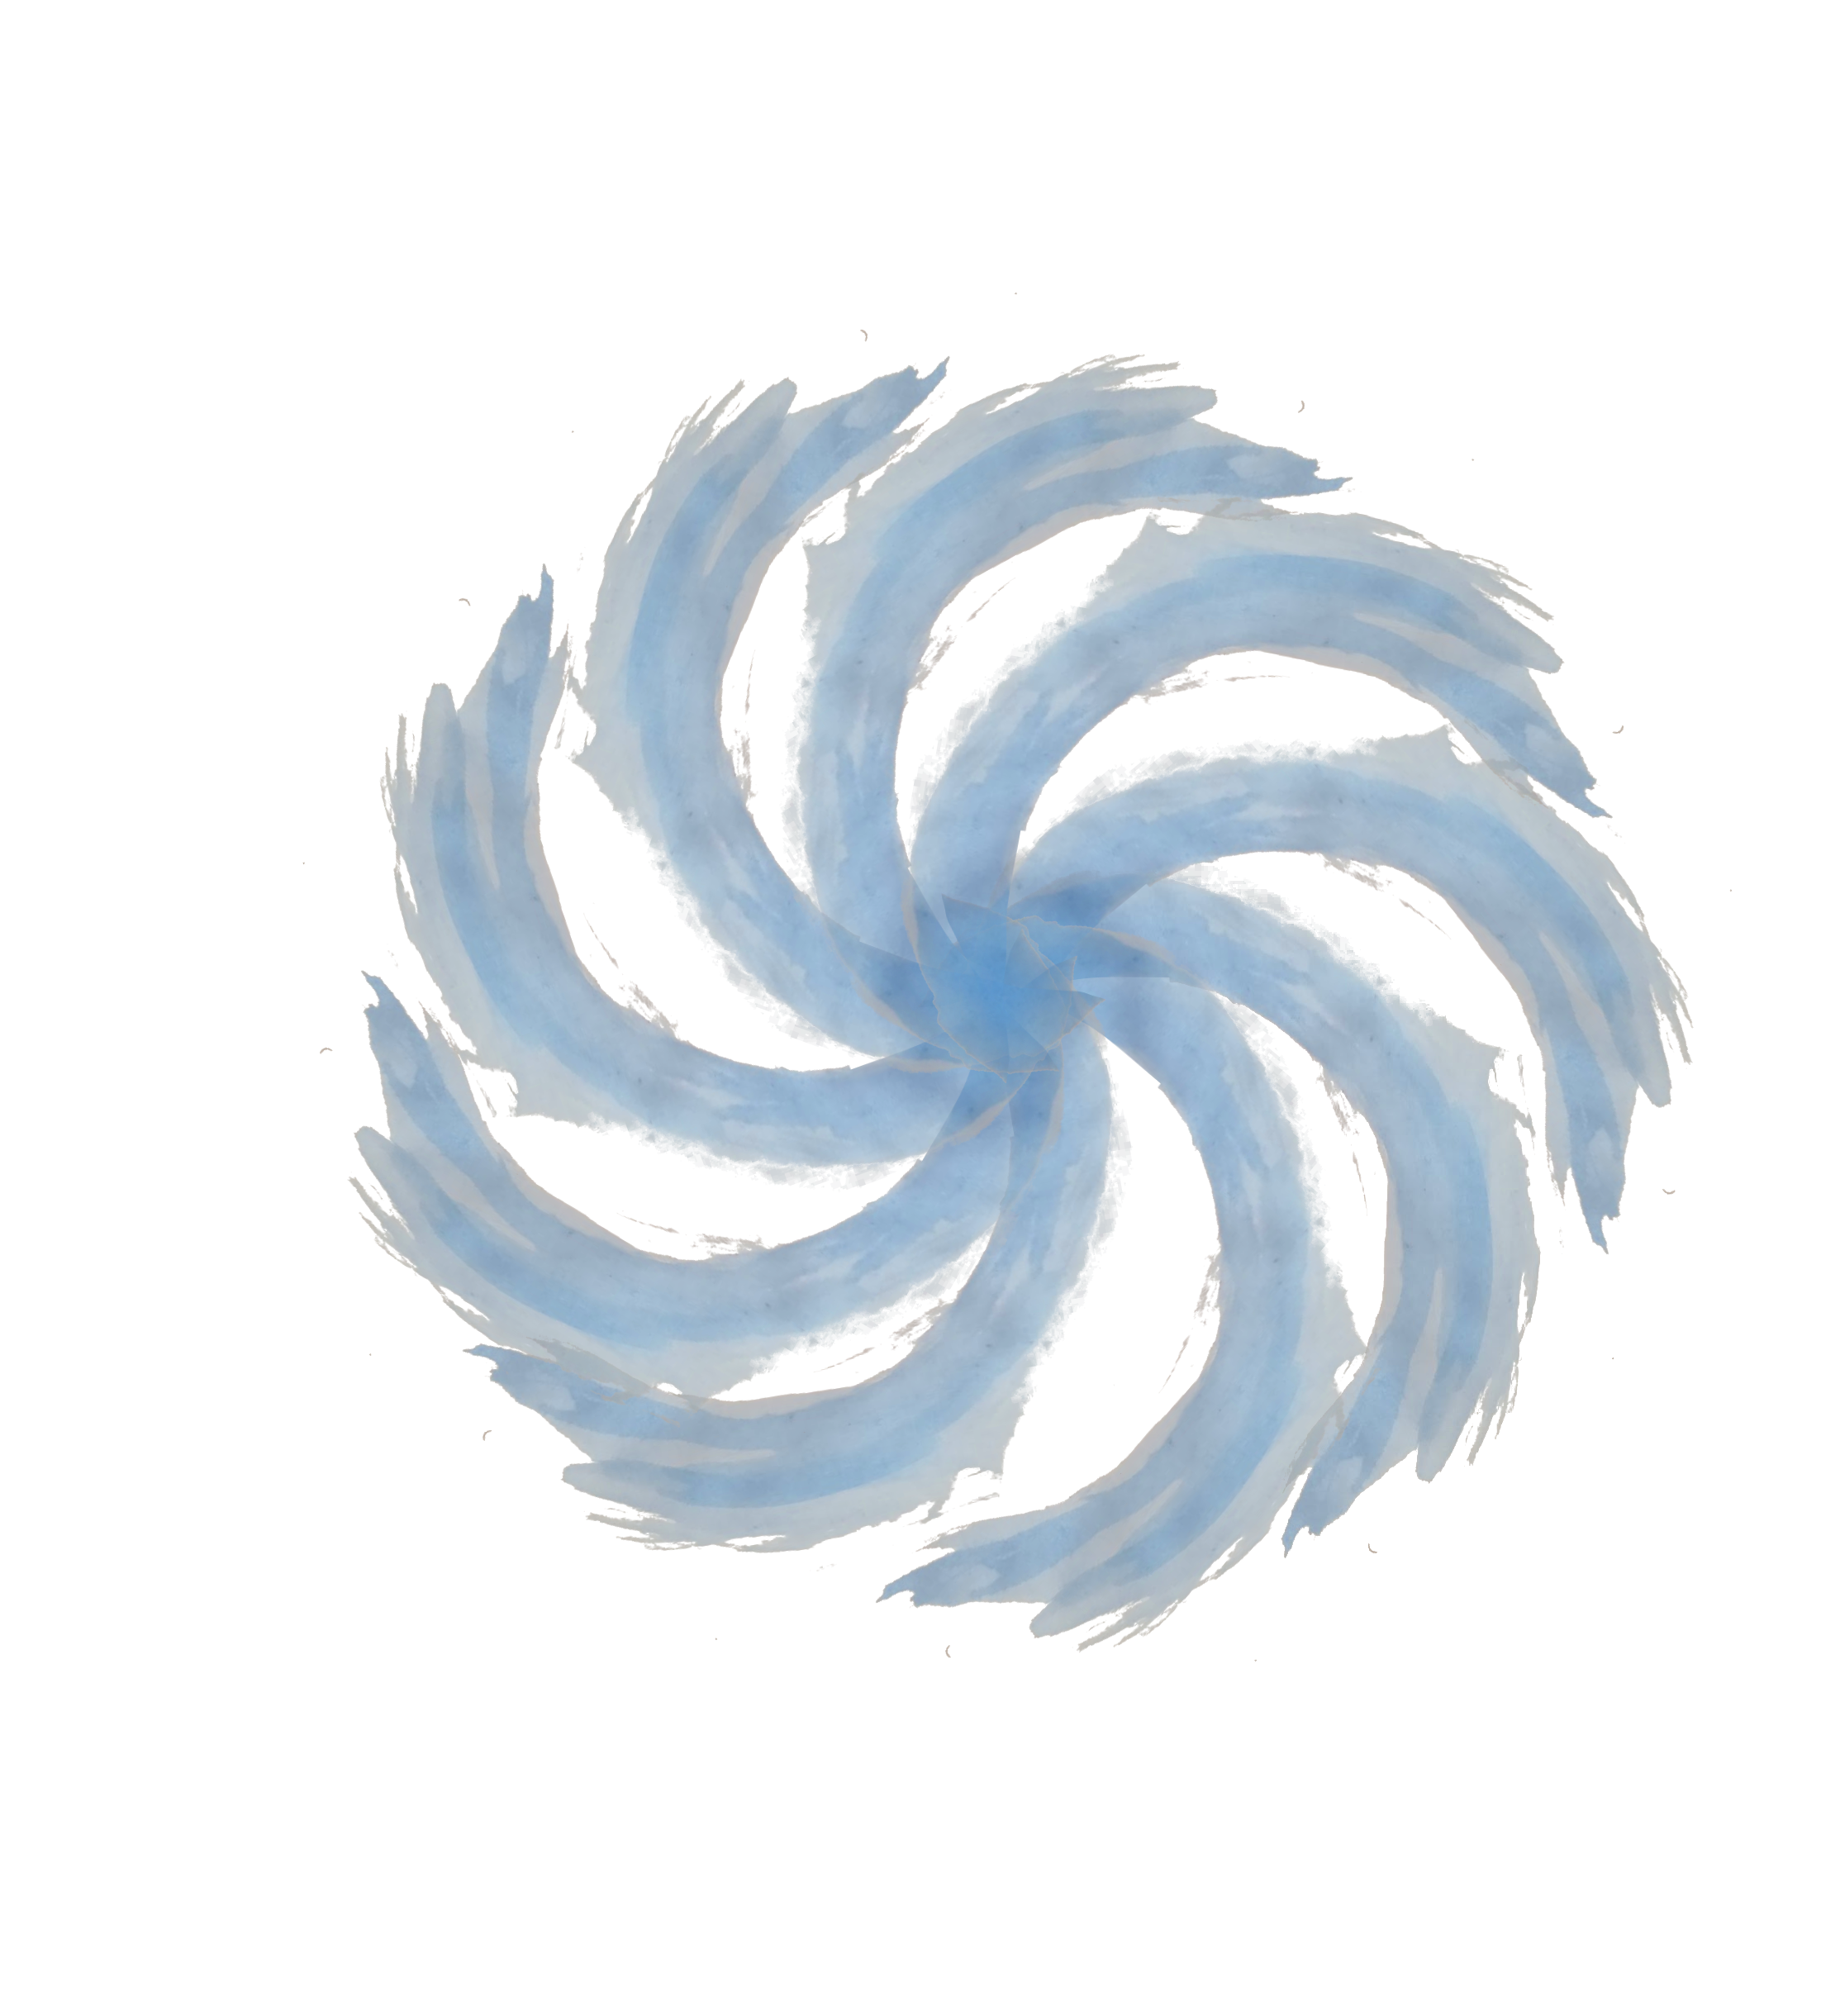
\includegraphics[width=.45\textwidth]{remolino3.png}};
		\end{tikzpicture}
%
%	\begin{tikzpicture}
%		\node[xscale=1,yshift=0cm] () {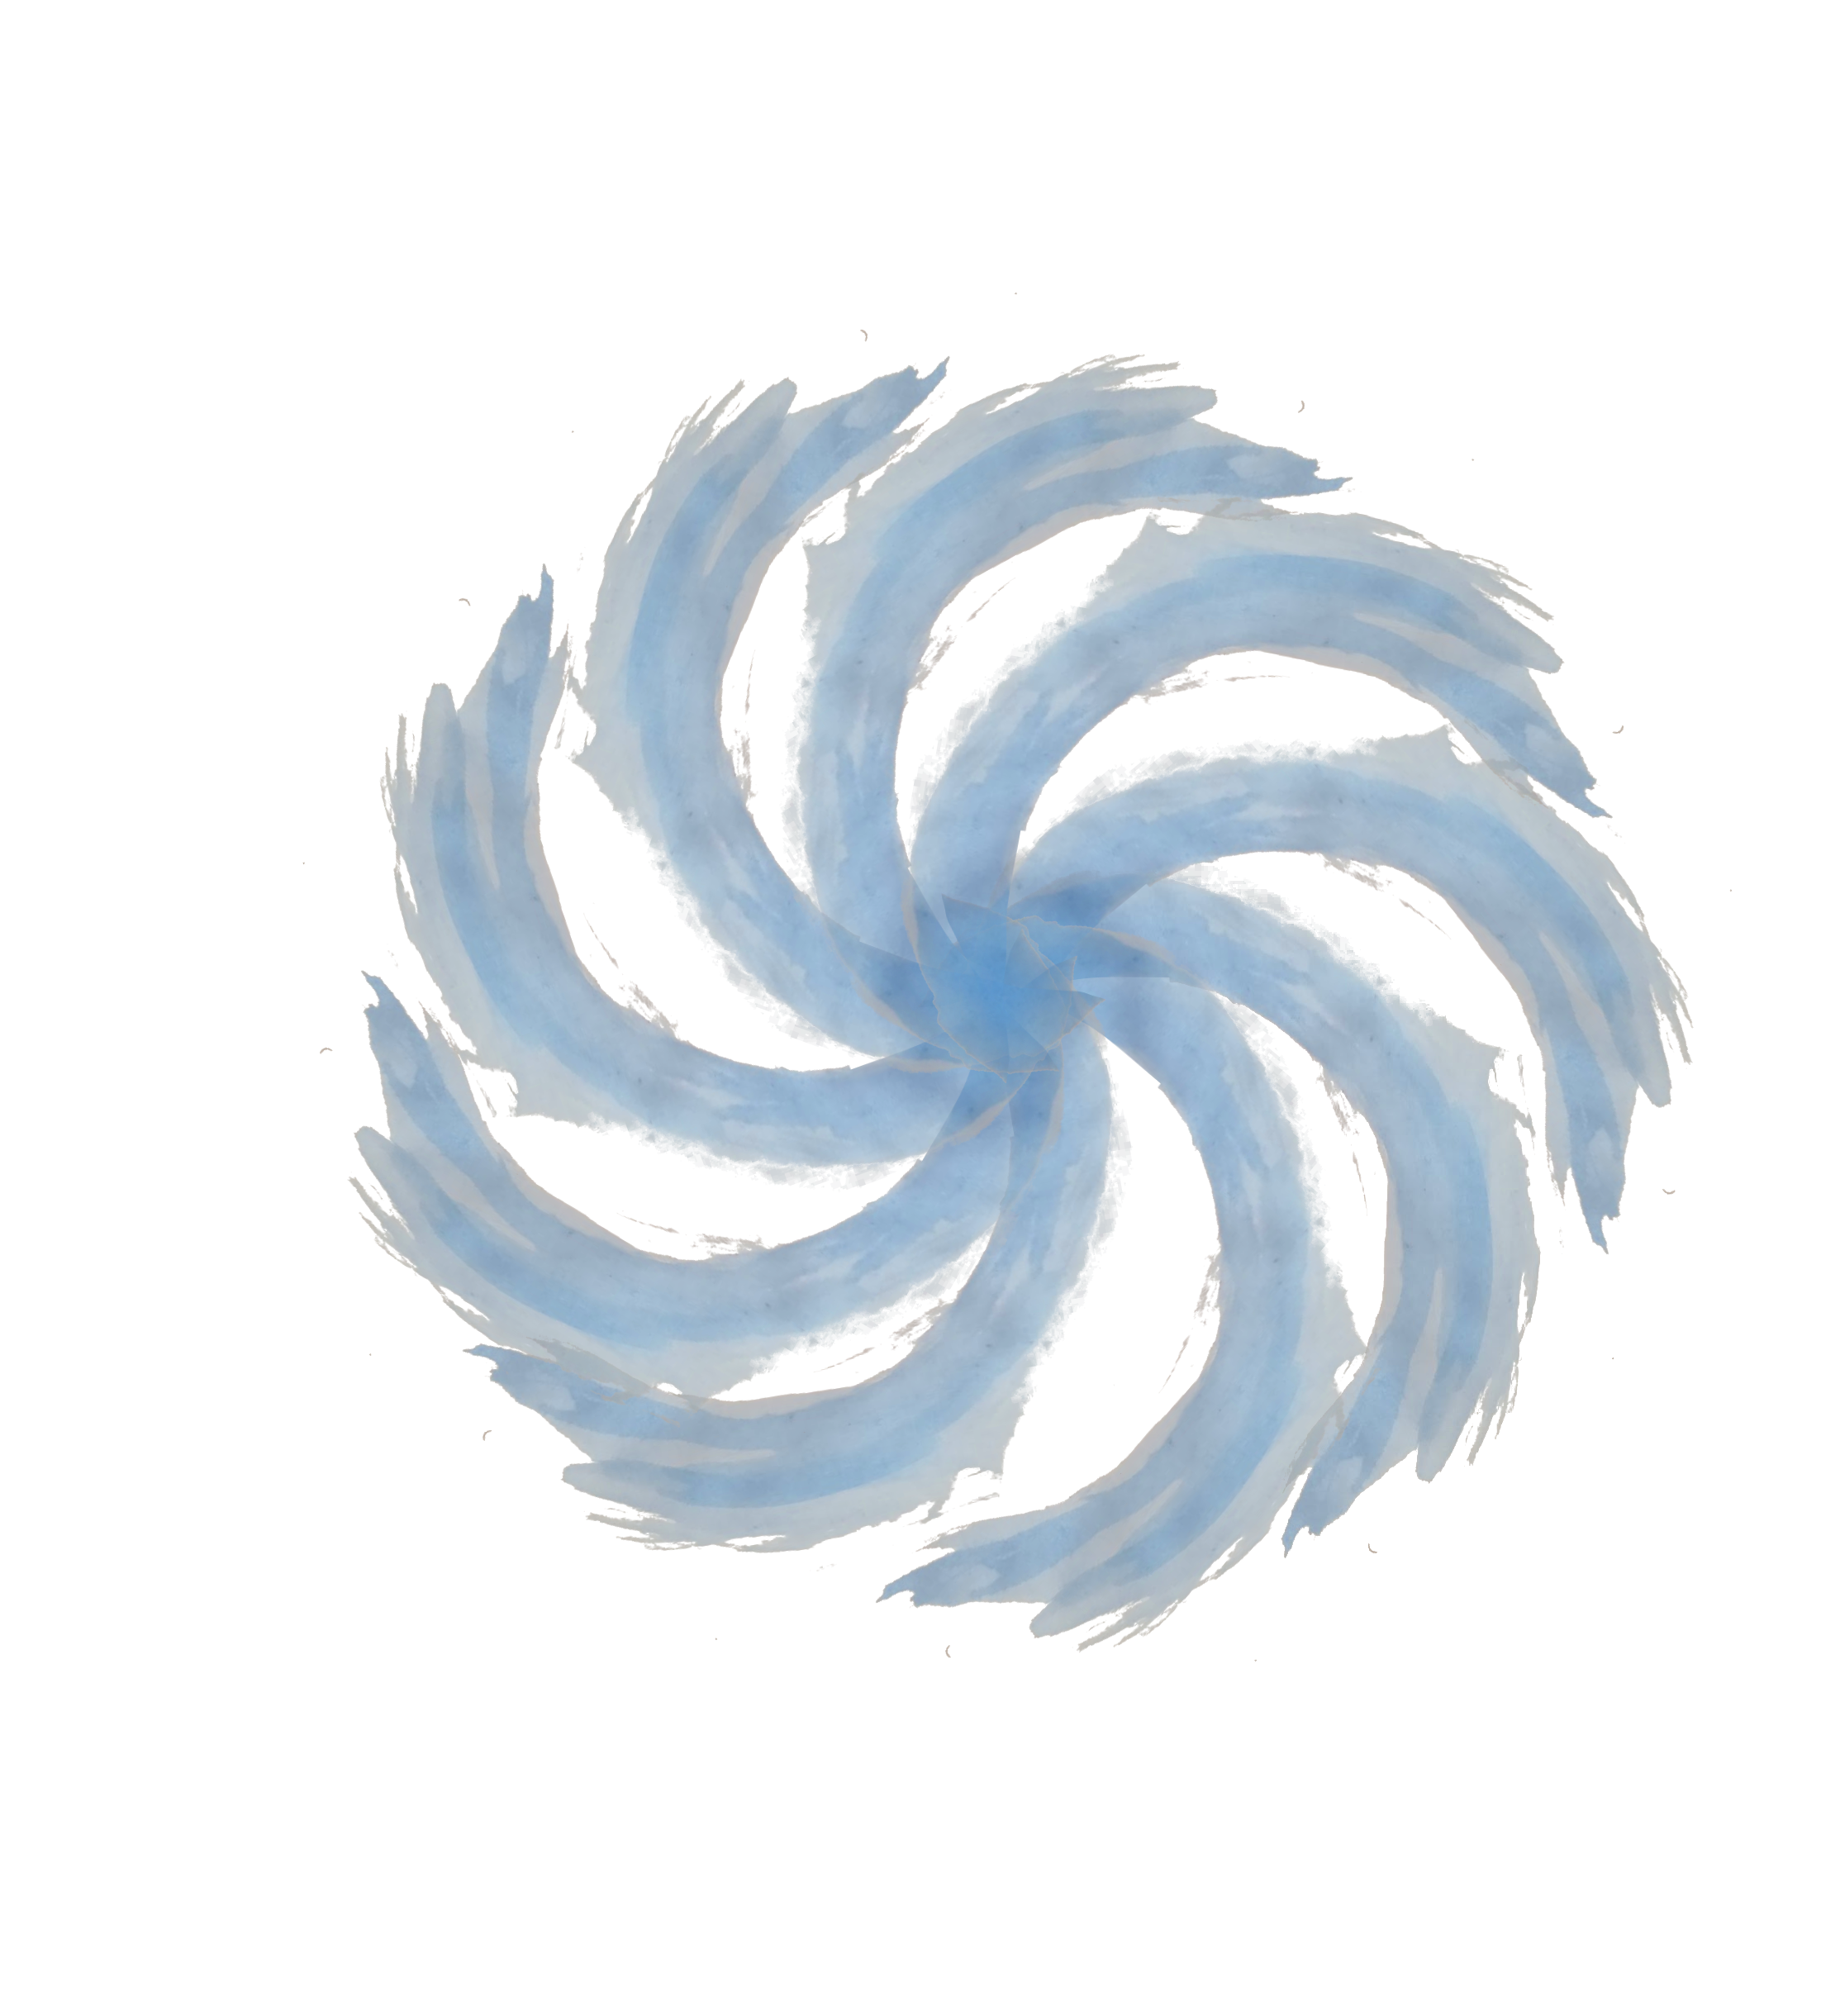
\includegraphics[width=.43\textwidth]{remolino3.png}};
%	\end{tikzpicture}
\end{wrapfigure}

ME GUSTA TAMBIÉN PENSAR EN QUE HAY UNA ESPECIE DE ATRACTOR QUE CONDUCE AQUELLO QUE ESTÁ LEJOS HACIA UN CENTRO. Y QUE AÚN CUANDO ALGÚN CAMINO PUEDA PARECER LEJANO, PRONTO ENCONTRAREMOS OTRO QUE NOS PUEDE CONDUCIR DE NUEVO AL MISMO CENTRO. EN ESTAS COSAS Y MÁS PENSABA MIRANDO LOS TRAZOS.

\newpage
\begin{tikzpicture}[remember picture, overlay]
	\node [inner sep=0pt, minimum width=\paperwidth, minimum height=\paperheight,opacity=1,color=Apricot] at (current page.center) {
\includegraphics[width=\paperwidth,height=\paperheight,angle=0]{paper30}};
\end{tikzpicture}
LOS TRAZOS TAMBIÉN SE DIBUJAN SI CAMINAMOS EN UNA CALESITA. 

\begin{wrapfigure} [12]{l}{.45\textwidth}\vspace{-1.2cm}%\hspace{-1.5cm}
	\begin{tikzpicture}
		\node[xscale=1,yshift=0cm] () {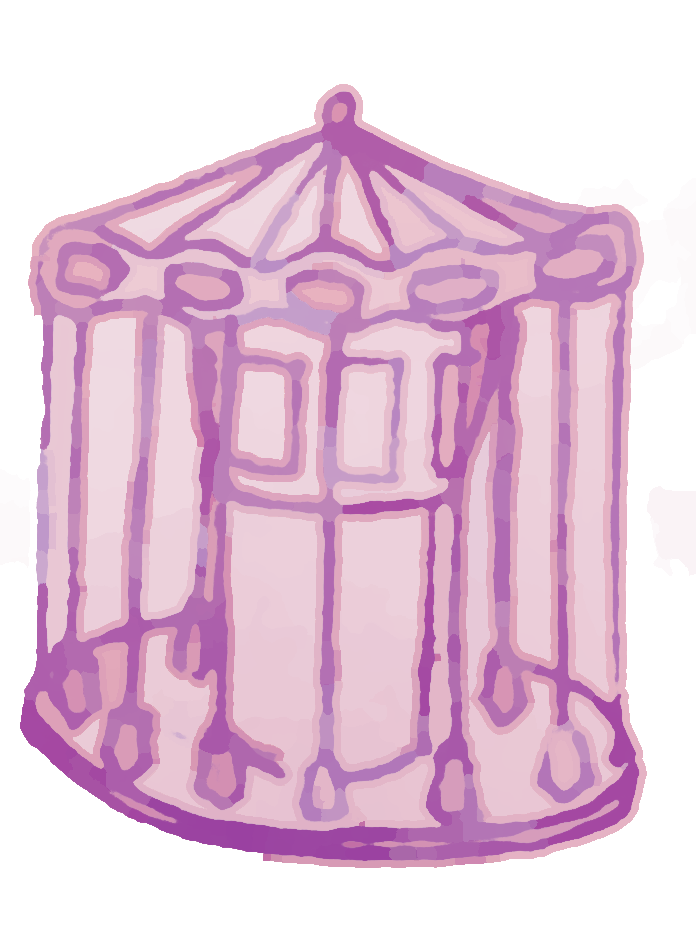
\includegraphics[width=.45\textwidth]{CALESITA1.png}};
	\end{tikzpicture}
\end{wrapfigure}

SI BIEN FUE  EN CASA QUE CONOCÍ PRIMERO LA SILLA GIRATORIA DE MI PAPÁ, PUDE VER QUE EN VARIAS PLAZAS DE BARRIO HAY MUY BELLAS CALESITAS QUE GIRAN CON EL MISMO PRINCIPIO. APRENDÍ QUE CUANDO NOS MOVEMOS SOBRE UN CÍRCULO EN ROTACIÓN, HAY UNA LIGERA FUERZA QUE NOS TIRA DESDE EL CENTRO HACIA AFUERA. LA LLAMAN ´´FUERZA CENTRÍFUGA´´. PERO HAY MUCHOS MÁS MISTERIOS ESCONDIDOS. 

DICE MI PAPÁ QUE SE PUEDE VIAJAR EN EL TIEMPO.

\newpage
\begin{tikzpicture}[remember picture, overlay]
	\node [inner sep=0pt, minimum width=\paperwidth, minimum height=\paperheight,opacity=1,color=Apricot] at (current page.center) {
\includegraphics[width=\paperwidth,height=\paperheight,angle=0]{paper30}};
\end{tikzpicture}

EN CALESITA, PODEMOS VIAJAR AL PASADO PERO NO A CUALQUIER MOMENTO AL AZAR. 

\begin{wrapfigure} [8]{l}{.45\textwidth}\vspace{-1.2cm}%\hspace{-1.5cm}
	\begin{tikzpicture}
		\node[xscale=1,yshift=0cm] () {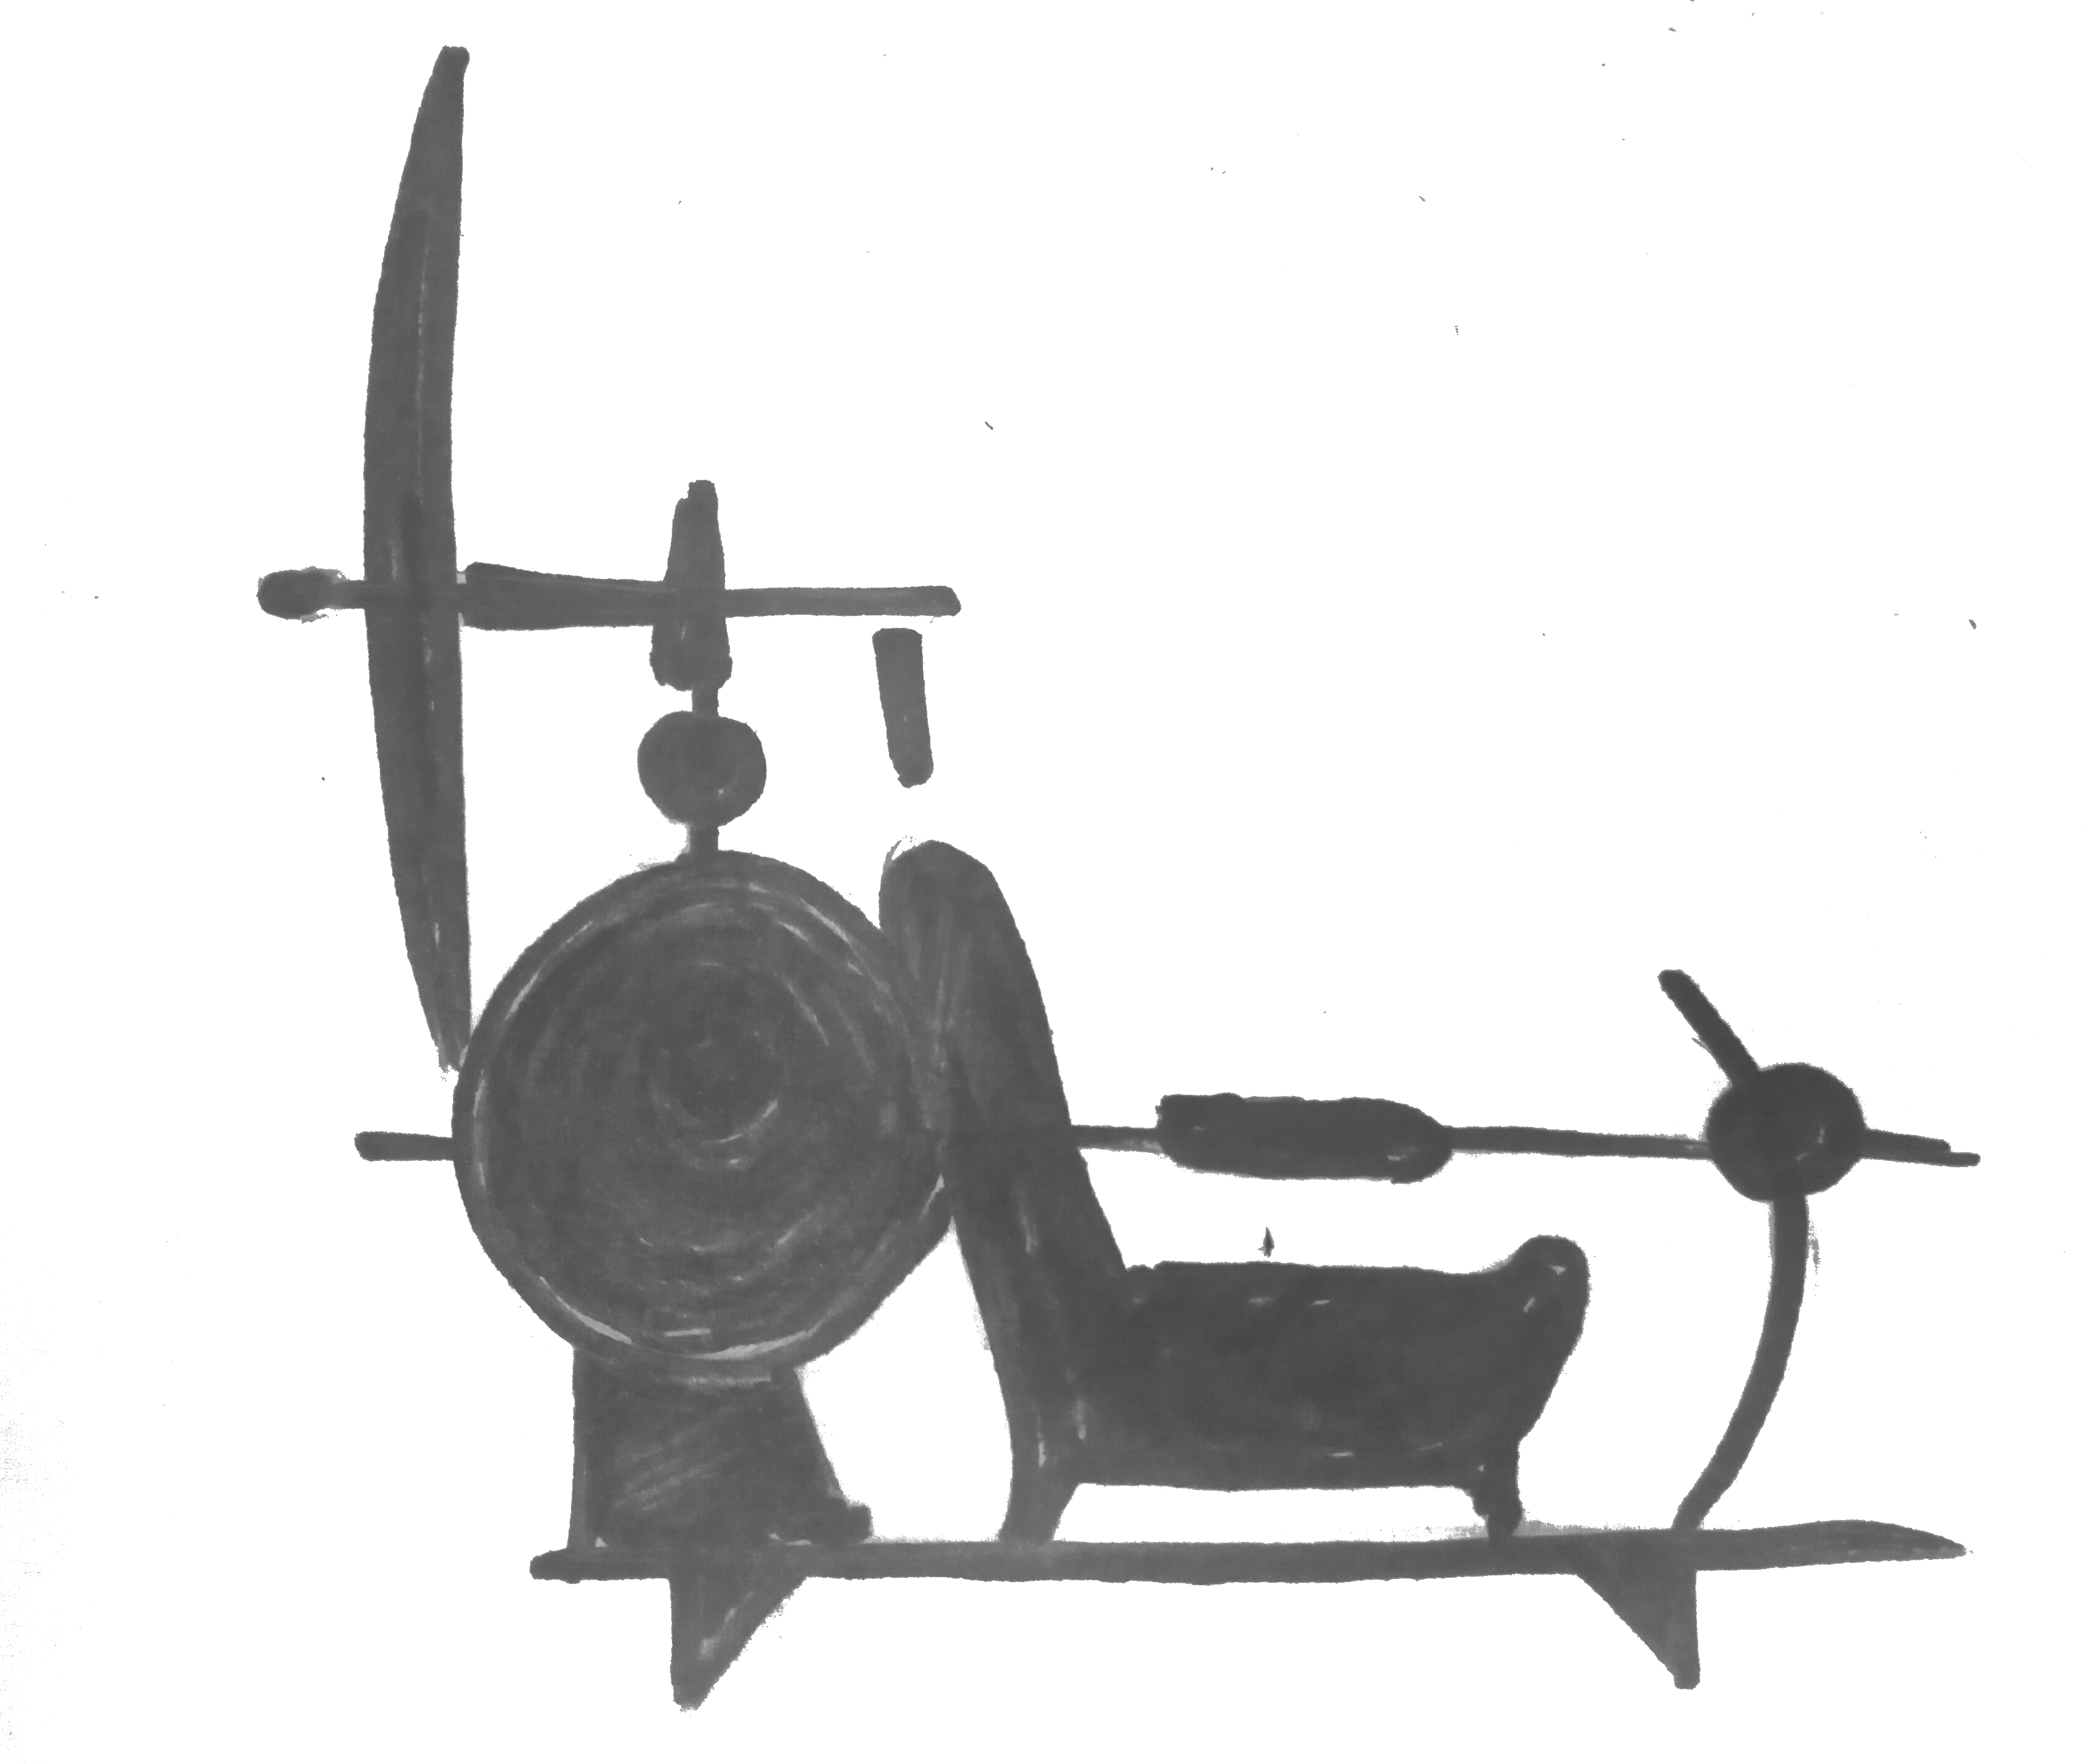
\includegraphics[width=.45\textwidth]{time_machine.png}};
	\end{tikzpicture}
\end{wrapfigure}

EN LA NOVELA, ´´LA MÁQUINA DEL TIEMPO´´, EL VIAJERO EN EL TIEMPO SE SUBÍA A UNA ESPECIE DE SILLÓN QUE TENÍA MUCHOS ELEMENTOS GIRATORIOS, DISCOS, ESFERAS, UNAS BARRAS DE MARFIL Y HASTA UNAS VARILLAS DE CUARZO. TODO SE DISPONÍA ALREDEDOR DE UN CÓMODO SILLÓN. DENTRO DE ESE APARATO, SE PODÍA ELEGIR EXACTAMENTE HASTA QUE AÑO VIAJAR Y A LA VELOCIDAD A LA QUE SE HACÍA.  

\newpage
\begin{tikzpicture}[remember picture, overlay]
	\node [inner sep=0pt, minimum width=\paperwidth, minimum height=\paperheight,opacity=1,color=Apricot] at (current page.center) {
\includegraphics[width=\paperwidth,height=\paperheight,angle=0]{paper30}};
\end{tikzpicture}
\begin{wrapfigure} [12]{l}{.45\textwidth}\vspace{-1.2cm}%\hspace{-1.5cm}
	\begin{tikzpicture}
		\node[xscale=1,yshift=0cm] () {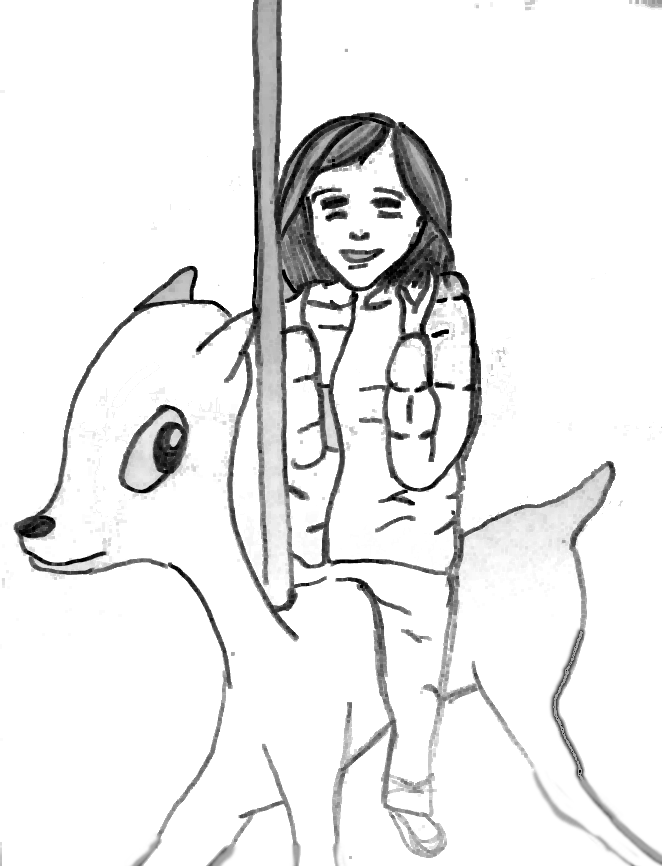
\includegraphics[width=.45\textwidth]{jeanne_bambi.png}};
	\end{tikzpicture}
\end{wrapfigure}
 
MUCHO MENOS SOFISTICADOS PERO NO MENOS IMPORTANTES ERAN LOS VIAJES DE LOS QUE ME HABLÓ MI PADRE CUANDO PASABA CERCA DE LA CALESITA DE VILLA DEL PARQUE. EL AIRE CON PERFUMES DE CARAMELO, LA MÚSICA RUTILANTE, LOS CHIRRIDOS DE ALGUNAS PIEZAS MECÁNICAS, EL GRITERÍO DE NIÑOS, LOS PRIMEROS SALUDOS DE LOS MÁS CHIQUITOS, LA EMOCIÓN DE SEPARARSE AUNQUE NO SEA UNA VUELTA Y TENER UNA BREVE AVENTURA SOLITOS$\ldots$ 

\newpage
\begin{tikzpicture}[remember picture, overlay]
	\node [inner sep=0pt, minimum width=\paperwidth, minimum height=\paperheight,opacity=1,color=Apricot] at (current page.center) {
\includegraphics[width=\paperwidth,height=\paperheight,angle=0]{paper30}};
\end{tikzpicture}
\begin{wrapfigure} [15]{l}{.65\textwidth}\vspace{-3.2cm}%\hspace{-1.5cm}
	\begin{tikzpicture}
		\node[xscale=1,yshift=0cm] () {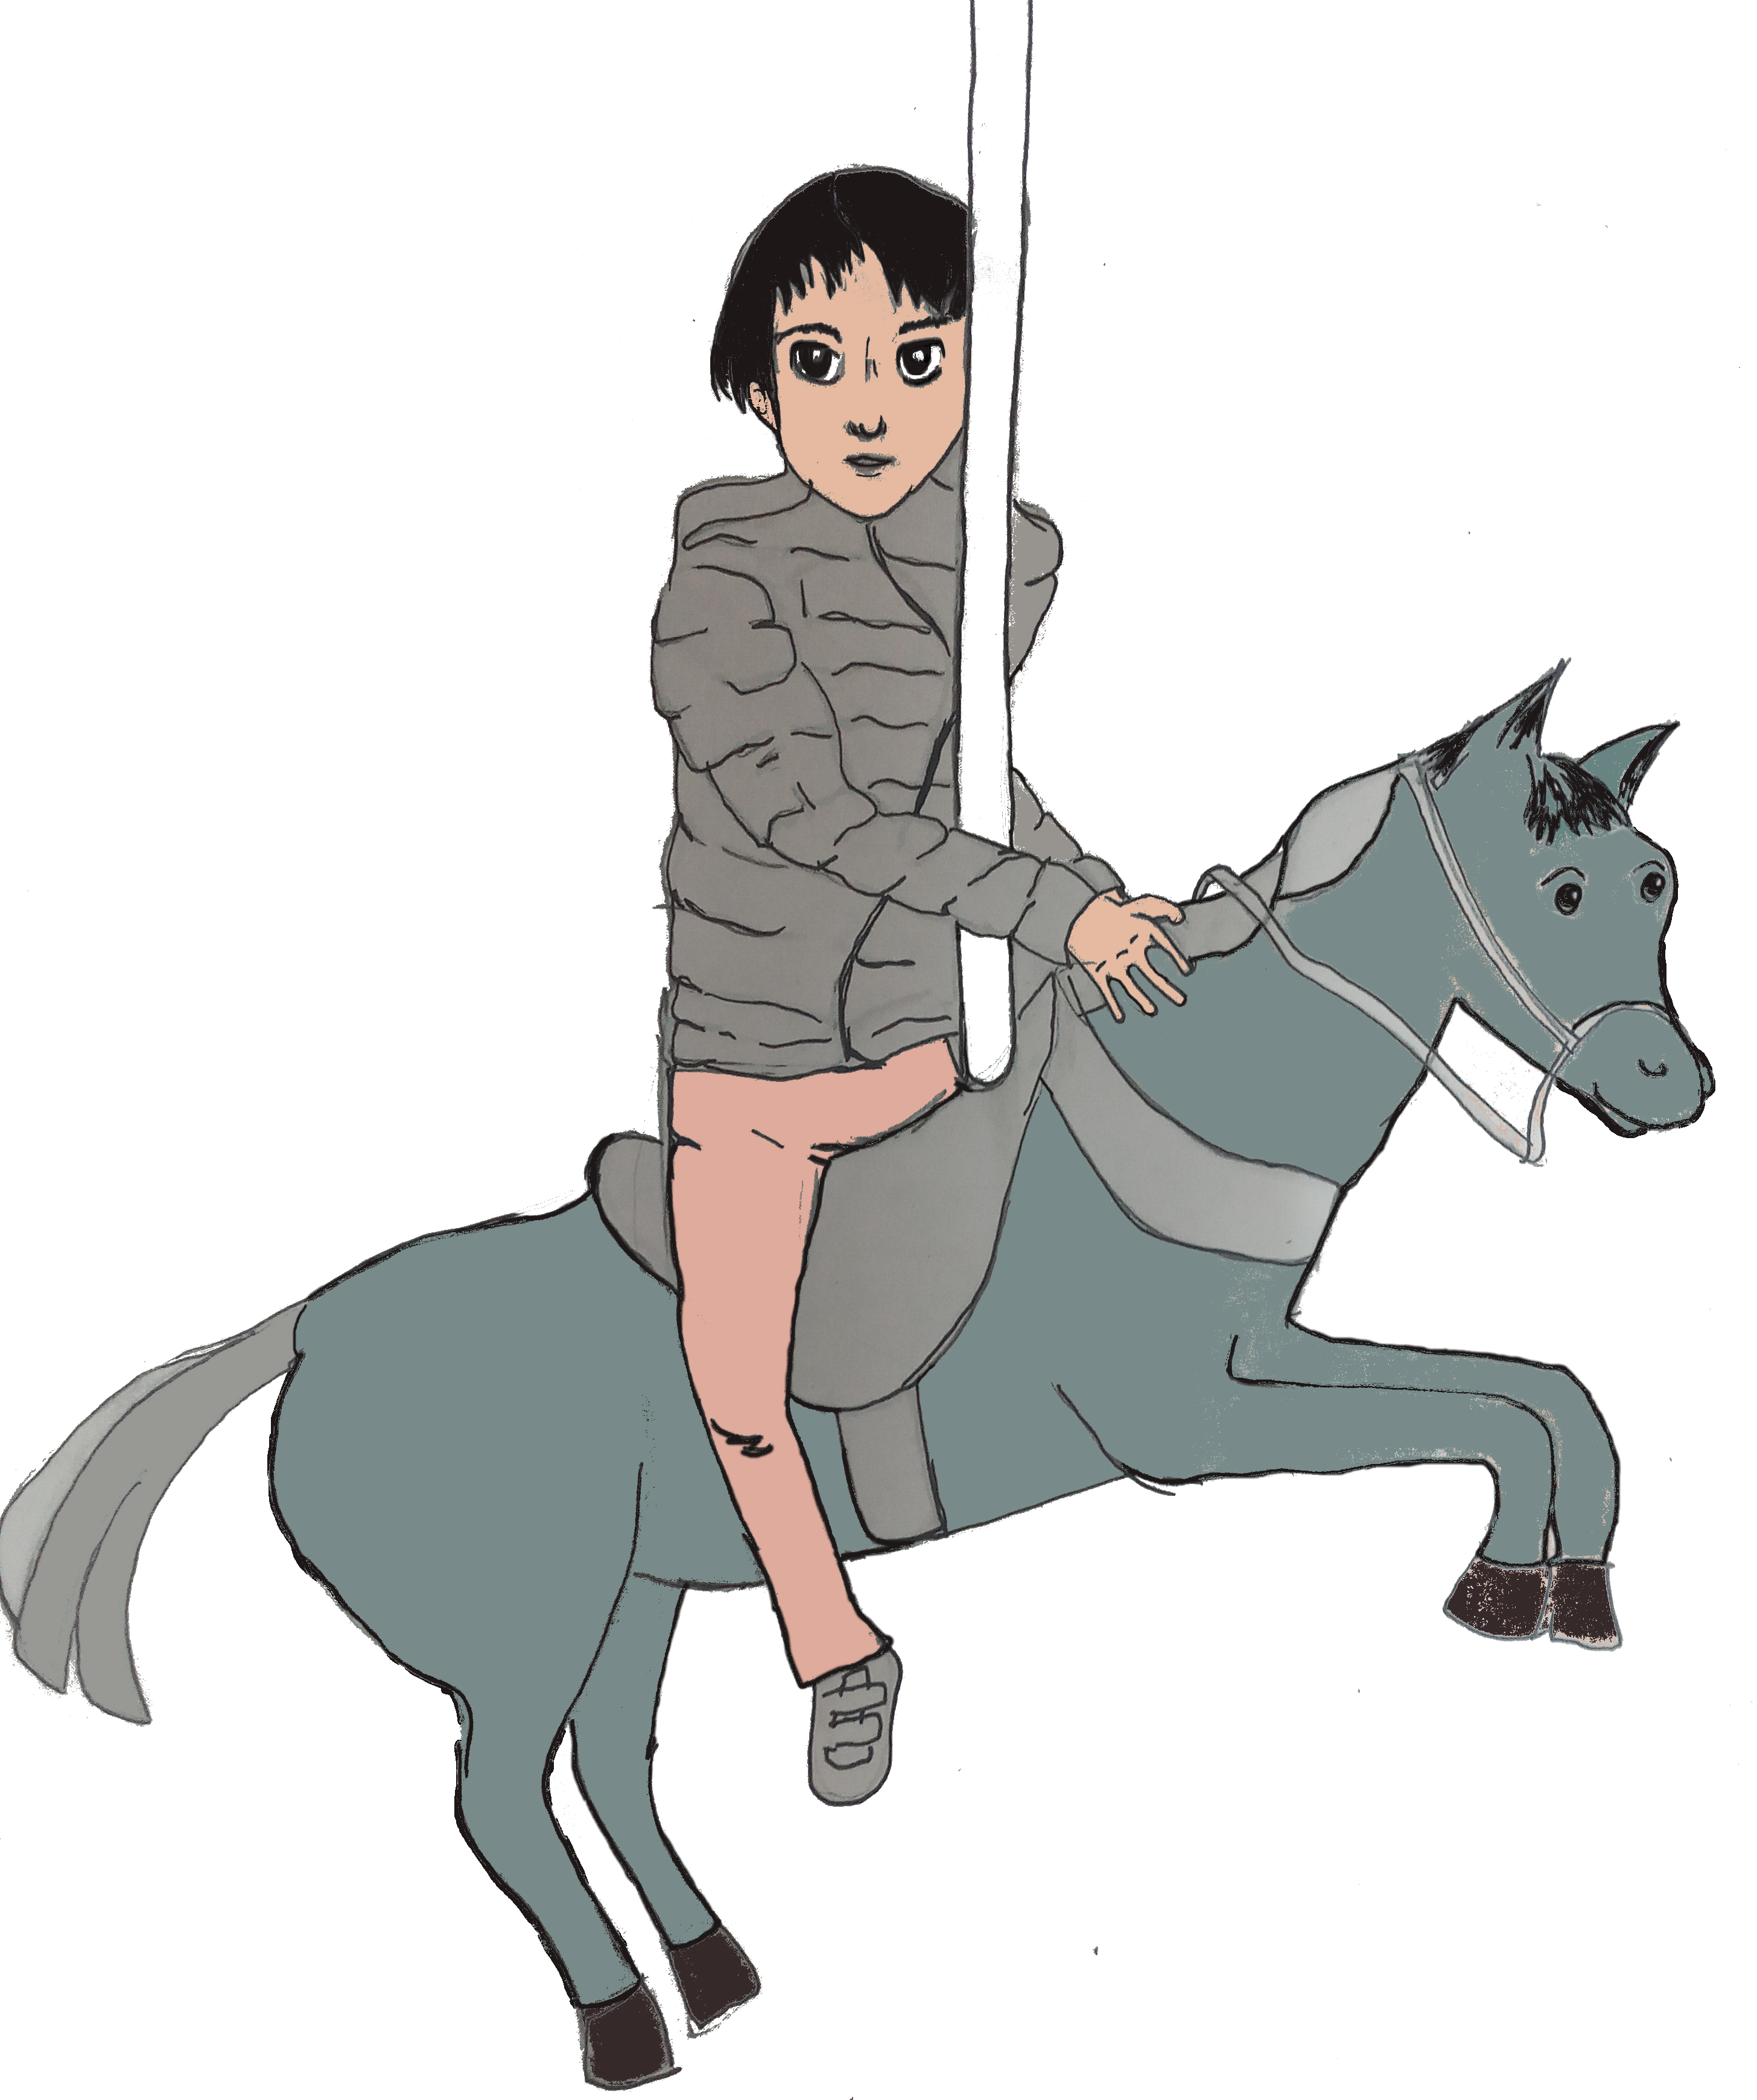
\includegraphics[width=.65\textwidth]{edmond_calesita_draw.png}};
	\end{tikzpicture}
\end{wrapfigure}
AUNQUE HAN TRANSCURRIDO MUCHAS VUELTAS DE CALESITA, SABE QUE 
ESAS Y OTRAS COSAS MÁS SIEMPRE ESTÁN VIVAS Y NUNCA DEJARÁN DE SALIR CON ALEGRÍA DE TANTOS MARAVILLOSOS RECUERDOS. 

\newpage
\begin{tikzpicture}[remember picture, overlay]
	\node [inner sep=0pt, minimum width=\paperwidth, minimum height=\paperheight,opacity=.5,color=Apricot] at (current page.center) {
\includegraphics[width=\paperwidth,height=\paperheight,angle=0]{paper30}};
\end{tikzpicture}
\begin{wrapfigure}[12]{r}{.4\textwidth}\vspace{-1.2cm}
	\begin{tikzpicture}
		\node[xscale=1,yshift=1cm] () {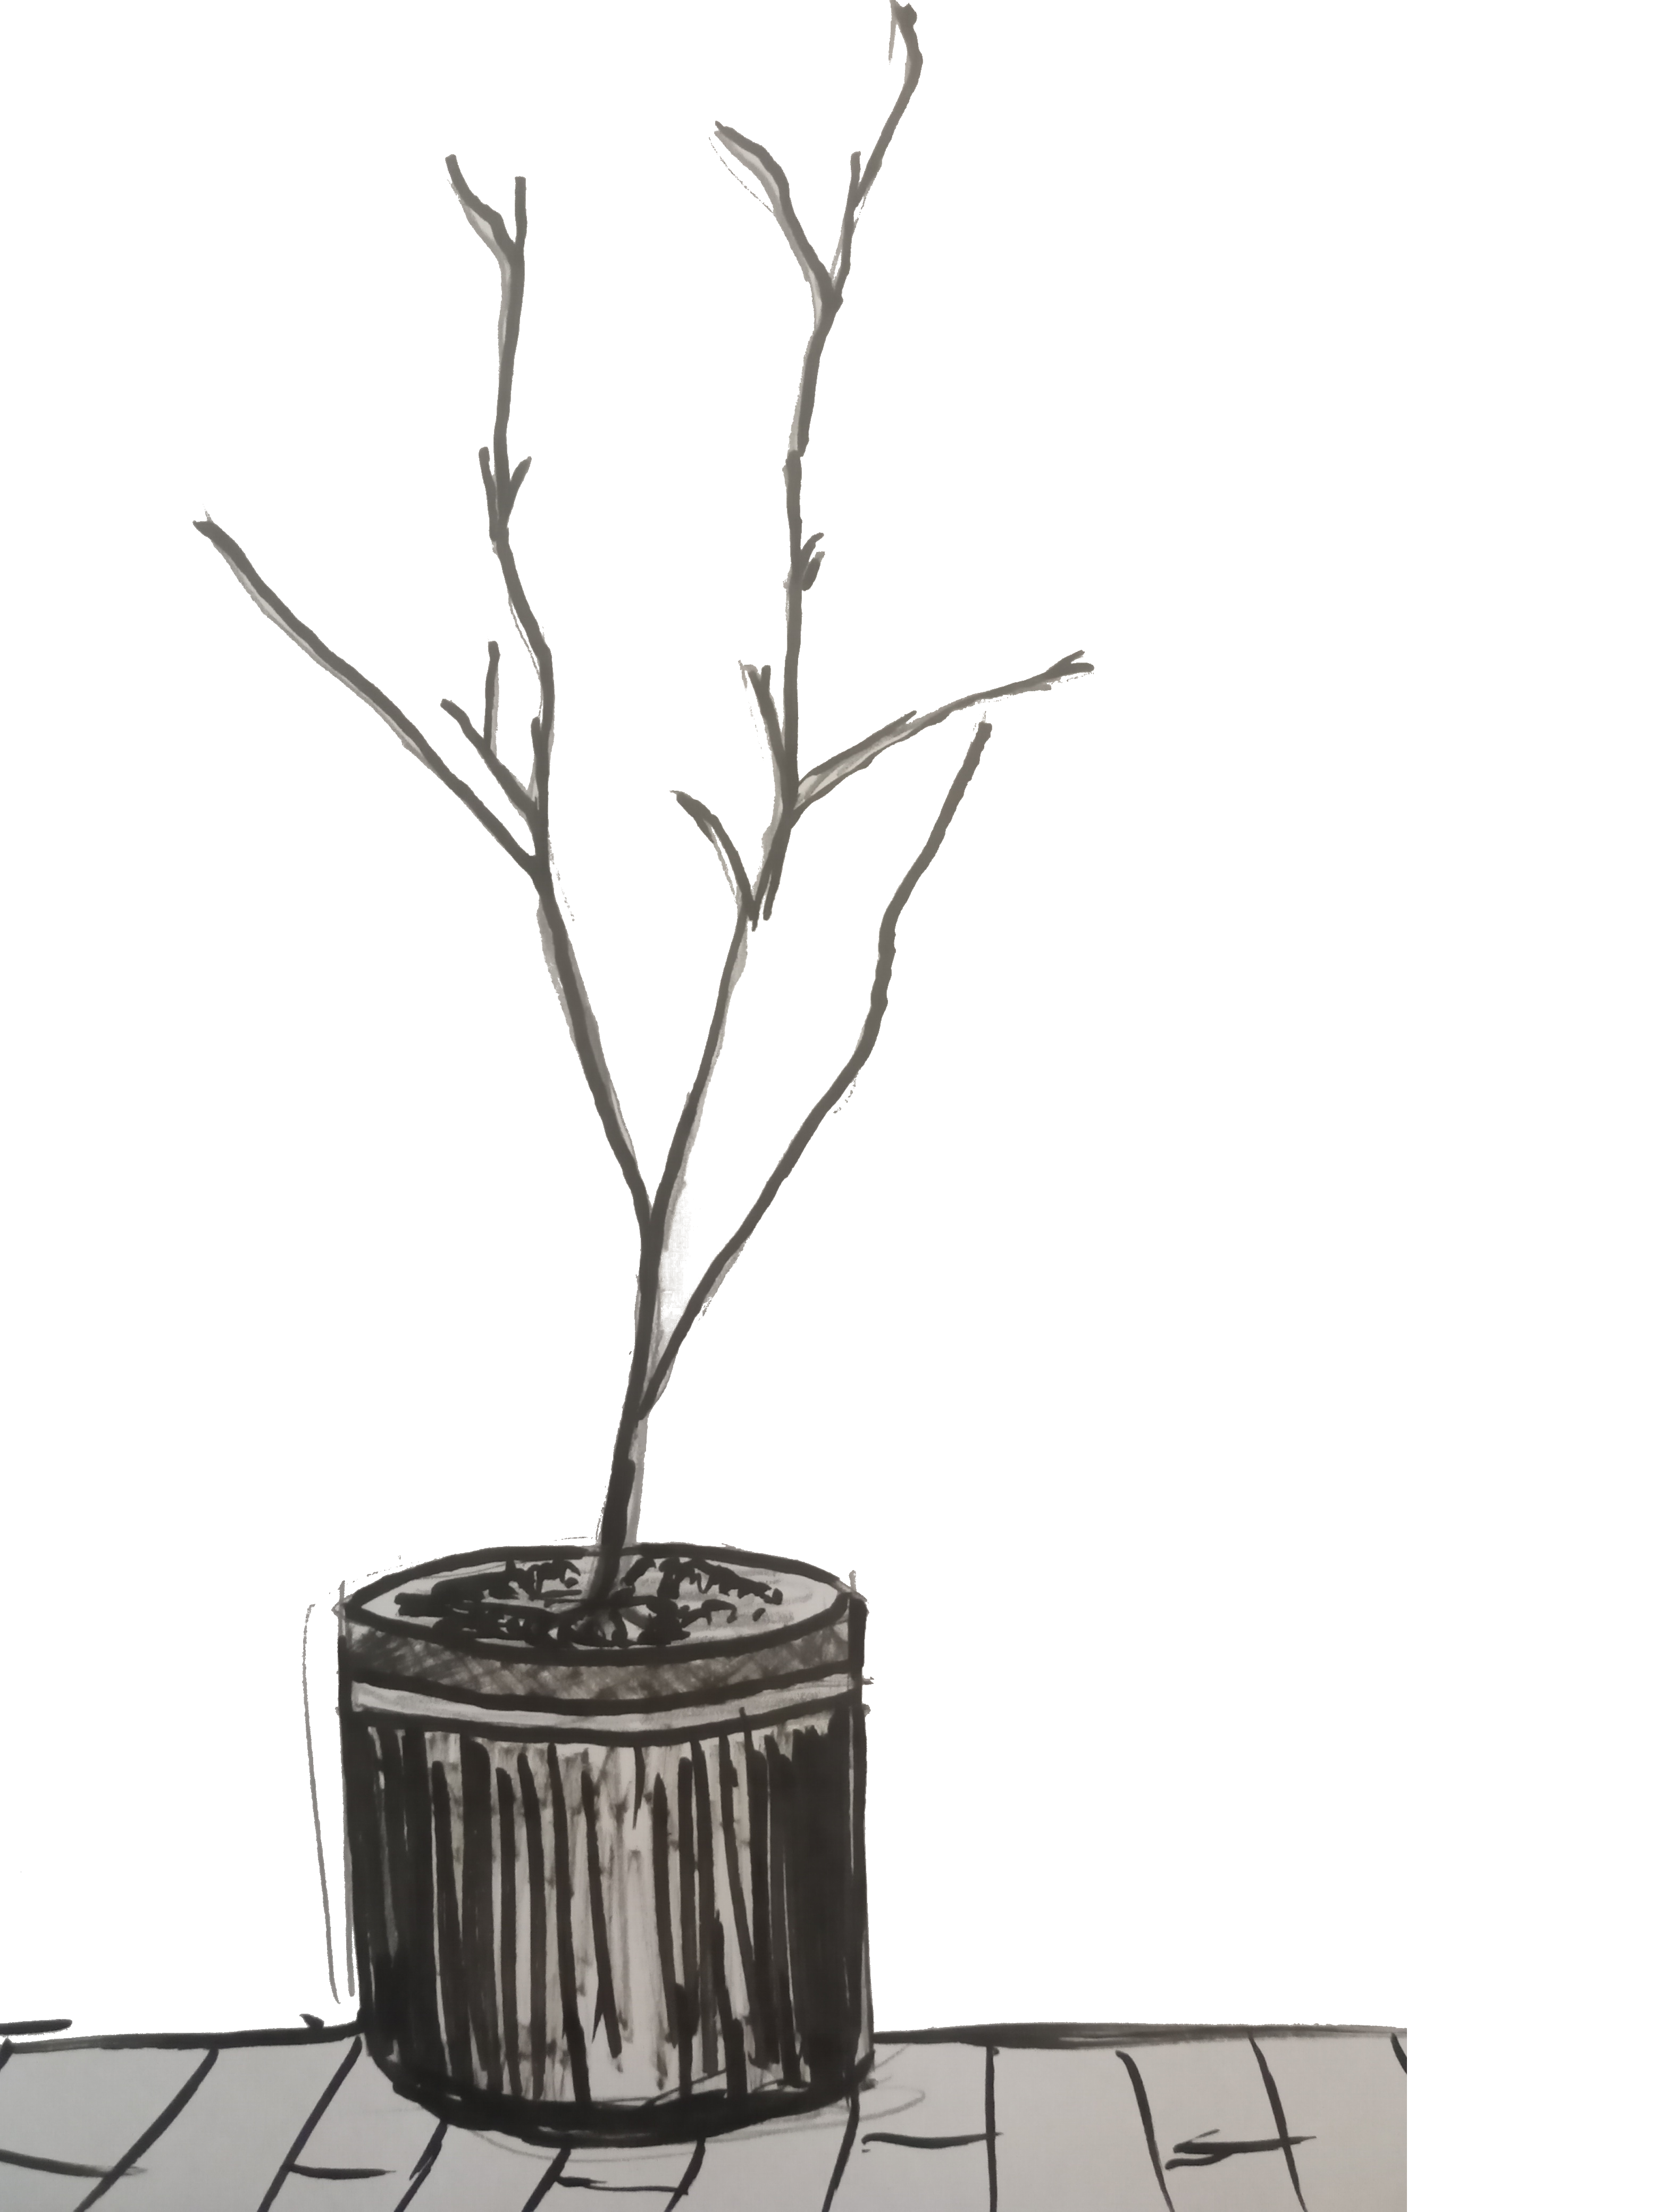
\includegraphics[width=.45\textwidth]{sakura_seco.png}};
	\end{tikzpicture}
\end{wrapfigure}
QUERÍA CONTARLES QUE ESTE INVIERNO, AÚN SI NO HA SIDO DEL TODO TAN FRÍO, RESULTÓ DURO PARA UNA DE MIS PLANTAS FAVORITAS, EL ARBOL DE SAKURA. SIEMPRE LO HEMOS CUIDADO, ES EL ÚNICO DE VEINTE SEMILLAS QUE LOGRÓ SOBREVIVIR Y ALCANZAR CIERTO TAMAÑO. DESGRACIADAMENTE, SÓLO  EN UN PAR DE NOCHES PERDIÓ PARTE DE SUS HOJAS MORDIDAS POR LA INVASIÓN DE UNAS HORMIGAS NEGRAS Y NUNCA PUDO RECUPERARSE DEL TODO.

\newpage
\begin{tikzpicture}[remember picture, overlay]
	\node [inner sep=0pt, minimum width=\paperwidth, minimum height=\paperheight,opacity=.7,color=Apricot] at (current page.center) {
\includegraphics[width=\paperwidth,height=\paperheight,angle=0]{paper30}};
\end{tikzpicture}
\begin{wrapfigure}[12]{r}{.35\textwidth}\vspace{-1.2cm}
	\begin{tikzpicture}
		\node[xscale=1,yshift=1cm] () {
\includegraphics[width=.4\textwidth]{ottoko_estudia}};
	\end{tikzpicture}
\end{wrapfigure}
TUVE QUE PONERME A ESTUDIAR A FONDO EL PROBLEMA. HAY ESPERANZA CUANDO LO INTENTAMOS CON ATENCIÓN Y DEDICACIÓN.

EL TEMA DE LAS HOJAS QUE MARCHITAN PUDO DEBERSE A FALTA DE HIERRO, PUES NO ES LO MISMO UN ÁRBOL EN MACETA, AUN SI ES UNA ENORME MACETAS, QUE AQUEL QUE CUENTA CON EL SOPORTE DE LA TIERRA LIBRE. SOLEMOS PONER COMPOST, LA DIGESTIÓN DE UNAS BUENAS LOMBRICES, PERO NO FUE SUFICIENTE. CONSEGUIMOS HIERRO DESDE UNA SAL COMERCIAL, EL SULFATO DE HIERRO, QUE TIENE UN COLOR VERDÁCEO. 

\newpage
\begin{tikzpicture}[remember picture, overlay]
	\node [inner sep=0pt, minimum width=\paperwidth, minimum height=\paperheight,opacity=.7,color=Apricot] at (current page.center) {};
 
\end{tikzpicture}
\begin{wrapfigure}[13]{l}{.4\textwidth}\vspace{-2cm}
	\begin{tikzpicture}
		\node[xscale=1] () {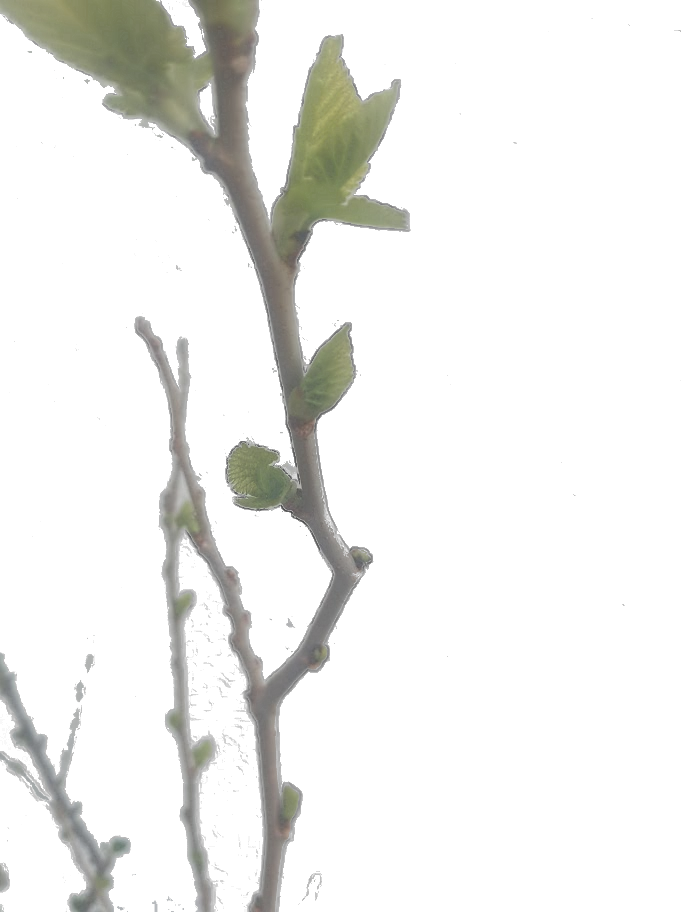
\includegraphics[height=.8\paperheight]{sakura_hojitas2}};
	\end{tikzpicture}
\end{wrapfigure}
PENSAMOS QUE EL POBRE ARBOLITO HABÍA DADO YA LO MEJOR DE SÍ. PERO LOS BUENOS CUIDADOS Y LA PRIMAVERA NOS DIERON UNA GRAN ALEGRÍA AL VER, PRIMERO, UNOS PUNTITOS VERDES DISTRIBUIDOS A LO LARGO DE LAS DÉBILES RAMAS.

Y UNOS DÍAS DESPUÉS EMPEZAMOS A VER, REPLEGADAS AÚN, LAS HOJITAS QUE SE AYUDARÁN A SALUDAR NUEVAMENTE AL SOL. PORQUE DESDE LA PACIENCIA Y EL AMOR, FLORECEN BELLAS LAS OPORTUNIDADES DE LA VIDA.
\newpage
\begin{tikzpicture}[remember picture, overlay]
	\node [inner sep=0pt, minimum width=\paperwidth, minimum height=\paperheight,opacity=.7,color=Apricot] at (current page.center) {
\includegraphics[width=\paperwidth,height=\paperheight,angle=0]{paper29}};
\end{tikzpicture}
\begin{wrapfigure}[13]{l}{.4\textwidth}\vspace{-2cm}\hspace{-3cm}
	\begin{tikzpicture}
		\node[xscale=1] () {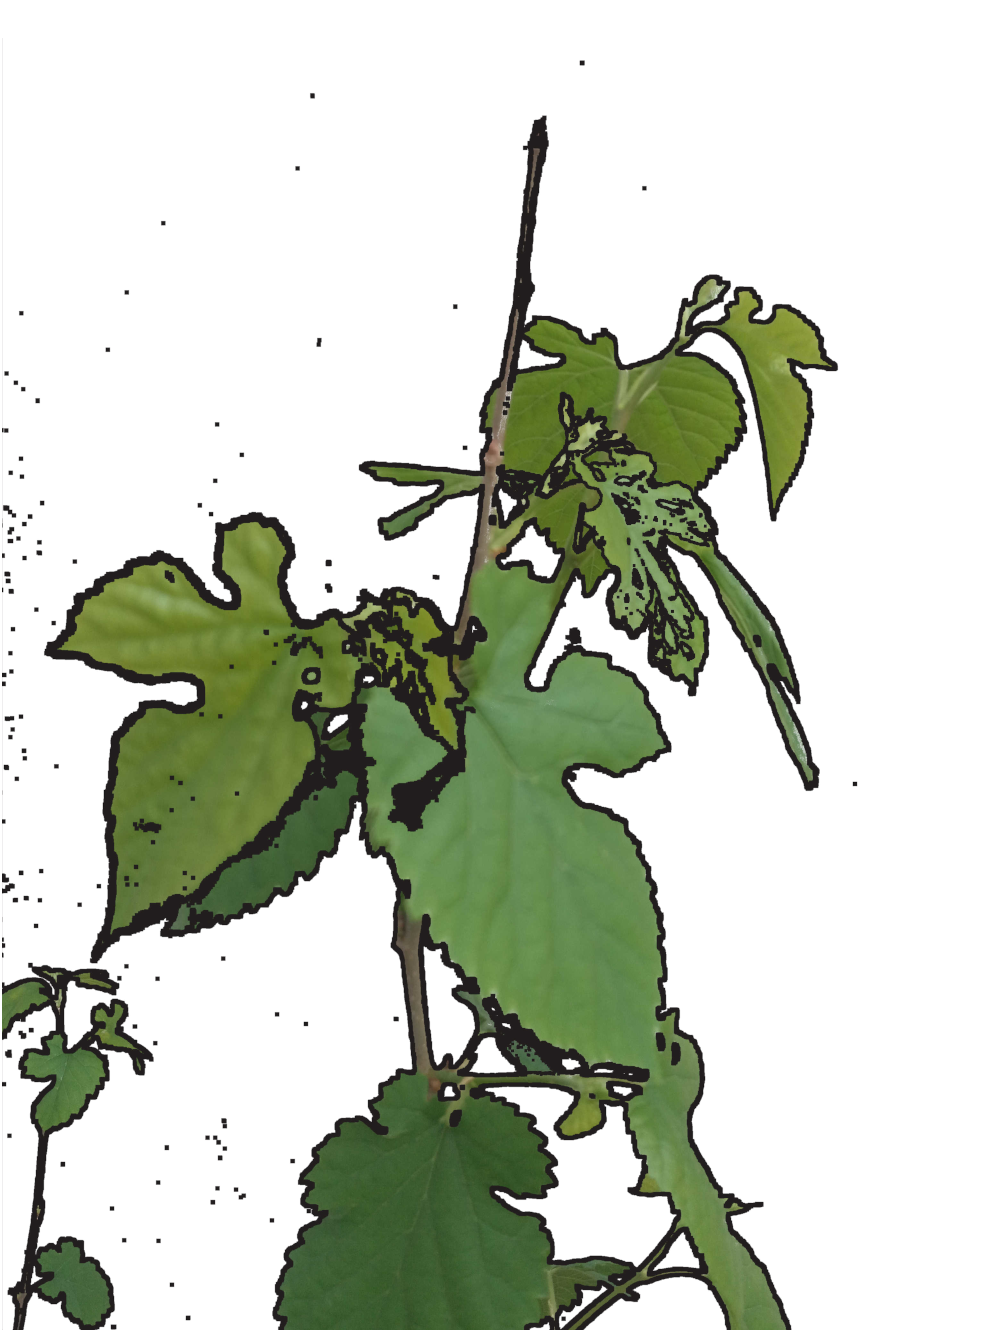
\includegraphics[height=.8\paperheight]{sakura_hojitas3.png}};
	\end{tikzpicture}
\end{wrapfigure}
Y ASÍ FUE QUE EL INVIERNO PASÓ Y DIÓ LUGAR A UNA HERMOSA PRIMAVERA. LOS BROTES Y HOJAS DEL SAKURA SE DESPLEGARON Y NO SÓLO VOLVIERON A SER TAN BELLAS COMO ANTES SINO QUE AÚN MÁS FRONDOSAS Y COLORIDAS. 

EL SAKURA TAMBIÉN NACIÓ EN EL 2021. FUE EN UNA PRIMAVERA ASÍ, AL MISMO TIEMPO QUE NOS CONOCIMOS.


QUERÍA CONTARLES ESO, ANTES DE ABORDAR MI FANTÁSTICA AVENTURA EN EL MUSEO.

\newpage
\begin{tikzpicture}[remember picture, overlay]
	\node [inner sep=0pt, minimum width=\paperwidth, minimum height=\paperheight,opacity=.7,color=Apricot] at (current page.center) {
\includegraphics[width=\paperwidth,height=\paperheight,angle=0]{paper29}};
\end{tikzpicture}
\begin{wrapfigure}[10]{r}{.35\textwidth}\vspace{-1.85cm}%\hspace{-3cm}
	\begin{tikzpicture}
		\node[] () {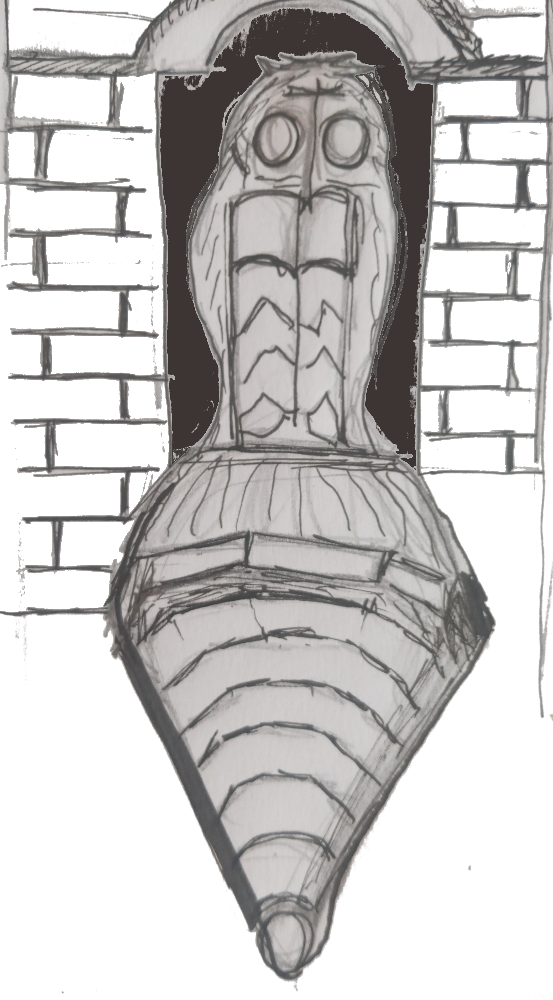
\includegraphics[scale=3.5]{lechuza2.png}};
	\end{tikzpicture}
\end{wrapfigure}
COMO MUCHAS DE LAS MEJORES HISTORIAS FELINAS, EN EL PRINCIPIO HUBO UN AVE. ESTA EN PARTICULAR ERA DE OJOS GRANDES, VIGILANTES, ALGO INTIMIDANTES Y HASTA ALCAHUETES, ME DIÓ LA IMPRESIÓN. SE HALLABA A UNA ALTURA CONSIDERABLE, Y SE 

MANTENÍA BIEN DERECHITA, PARECÍA SER LA GUARDIANA DE UN LUGAR MUY ESPECIAL. Y TENÍA UNA COMPAÑERA IDÉNTICA UBICADA A TAN SÓLO UNOS METROS. DIJE DERECHITA PERO MÁS BIEN LA NOTÉ RÍGIDA, TARDE UN MOMENTO EN DARME CUENTA DE QUE ERAN DOS ESTATUAS. AMBAS SE UBICABAN A LOS LADOS DE UNA ENORME PUERTA DE HIERRO.
\newpage
\begin{tikzpicture}[remember picture, overlay]
	\node [inner sep=0pt, minimum width=\paperwidth, minimum height=\paperheight,opacity=1] at (current page.center) {
\includegraphics[width=\paperwidth,height=\paperheight,angle=0]{paper29}};
\end{tikzpicture}
\begin{minipage}[l]{.45\textwidth}\hspace{-2cm}
 \begin{tikzpicture}
 	\node[] () {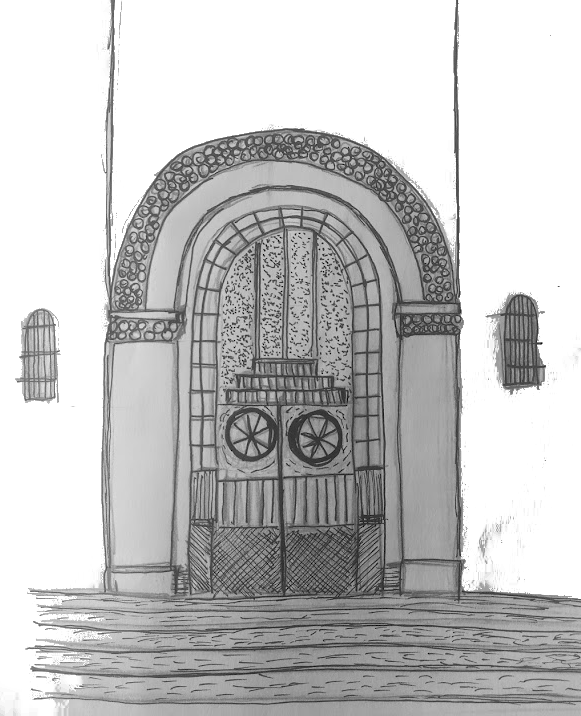
\includegraphics[height=.9\textheight]{puerta_museo1.png}};
 \end{tikzpicture}
\end{minipage}
\begin{minipage}[r]{.45\textwidth}
UNA PUERTA SEMEJANTE FORZOSAMENTE GUARDARÍA ASUNTOS MUY IMPORTANTES. SECRETOS DE MILES Y MILLONES DE AÑOS ATRÁS. UN UNIVERSO DE CIENCIA Y CULTURA, EN FIN EL TRABAJO IDEAL PARA UN FELINO SAGAZ Y DECIDIDO!
\end{minipage}
 
\newpage
\begin{tikzpicture}[remember picture, overlay]
	\node [inner sep=0pt, minimum width=\paperwidth, minimum height=\paperheight,opacity=.4] at (current page.center) {
\includegraphics[width=\paperwidth,height=\paperheight,angle=0]{paper29}};
\end{tikzpicture}
-  ´´FELIS SILVESTRIS CATUS!!´´, EXCLAMÓ UNA VOZ JOVEN, ESTUDIOSA Y ENTUSIASTA.

-  ´´AGARREN A ESE GATO ROÑOSO!´´, VOCIFERÓ OTRA, MADURA, DIRECTIVA Y SIN MUCHA PACIENCIA, 

- ´´ESE GATITO NEGRO NO PAGÓ ENTRADA, PAPÁ!´´ DIJO DIVERTIDA UNA NENA.

ACELERÉ CON TODAS MIS FUERZAS Y ATRAVESÉ EL HALL CENTRAL. EL PISO DE MOSAICO GRANÍTICO, CAMINADO POR MILES Y MILES DE PERSONAS A LO LARGO DE TANTOS AÑOS, ERA LISO, CLARO Y POR SUPUESTO, RESBALOSO PARA LAS PATAS DE UN GATO. AL GIRAR Y EVITAR CUALQUIER INTENTO POR DETENERME, MIS PATAS TRASERAS QUEDARON PATINANDO CON LIGEREZA. 

EN UN PESTAÑAR DE OJOS FELINOS, DECIDÍ DIRIGIRME HACIA UNA SALA OSCURA, ALLÍ DONDE LOS SENTIDOS HUMANOS SON TORPES.
 
\newpage
\begin{tikzpicture}[remember picture, overlay]
	\node [inner sep=0pt, minimum width=\paperwidth, minimum height=\paperheight,opacity=.4] at (current page.center) {
\includegraphics[width=\paperwidth,height=\paperheight,angle=0]{paper31}};
\end{tikzpicture}
\begin{wrapfigure}[8]{r}{.45\textwidth}\vspace{-1.25cm}%\hspace{-3cm}
	\begin{tikzpicture}
		\node[] () {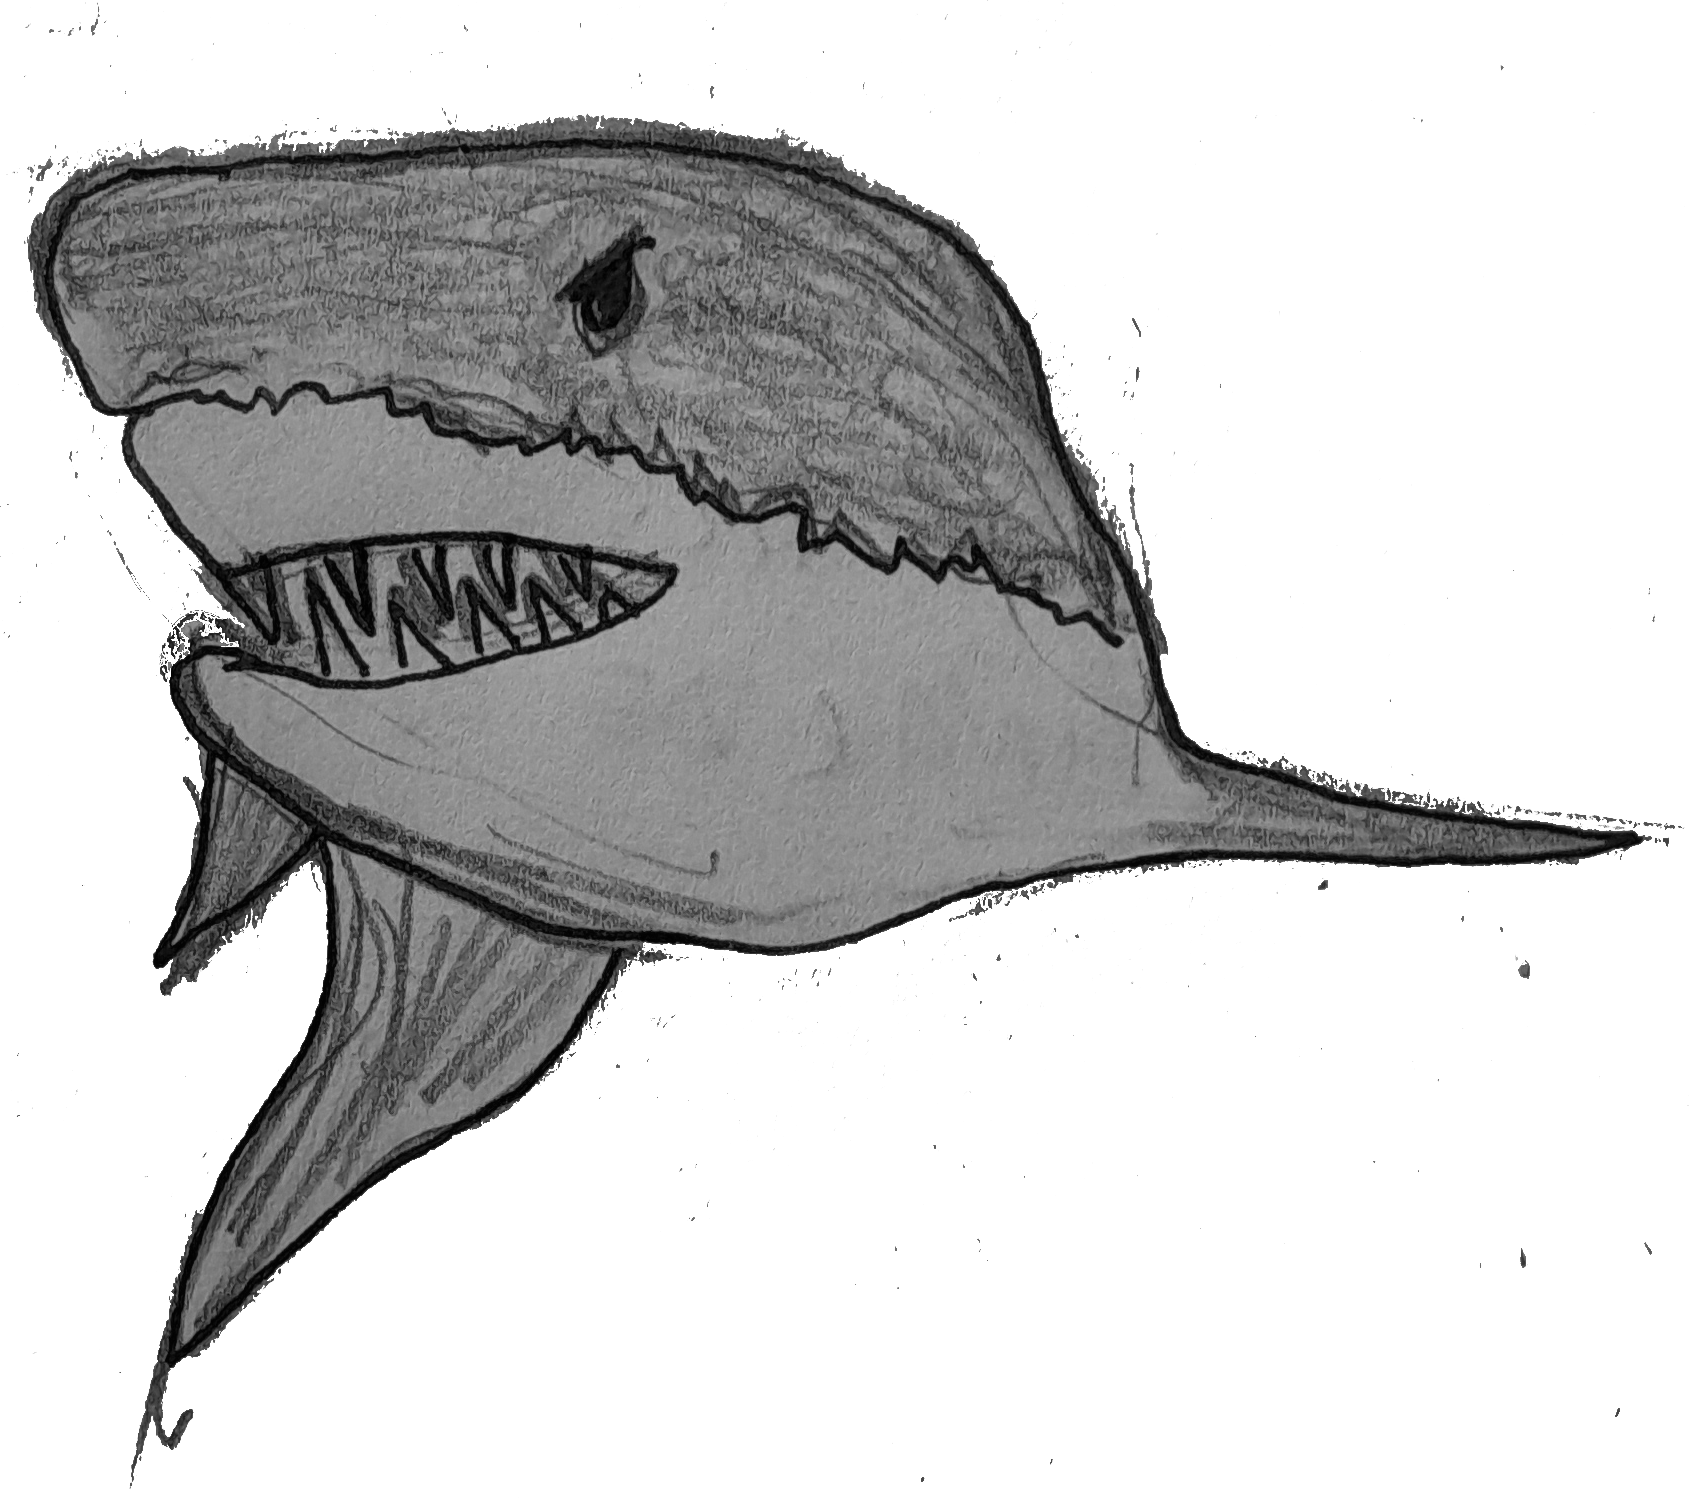
\includegraphics[width=\linewidth]{tiburon.png}};
	\end{tikzpicture}
\end{wrapfigure}
MÀS QUE UNA SALA, SE TRATABA DE UN ENORME CORREDOR DONDE HABÍA GRANDES PECERAS ILUMINADAS. SE VEÍAN PECES DE DISTINTOS, TAMAÑOS, FORMAS Y COLORES. NADA SE MOVÍA EN LA ESCENA PERO DABA LA SENSACIÓN DE QUE ESTABAN VIVOS, SE LLAMAN DIORAMAS. ME QUEDÉ UN RATO TRANQUILO MIRANDO DESDE UN COSTADO SIN LUZ DONDE NADIE ME PODÍA VER.

EN UNA REPRESENTACIÓN DEL FONDO DEL MAR, ME LLAMÓ LA ATENCIÓN UN ENORME DEPREDADOR, EL TIBURÓN. OBSERVÁNDOLO A DISTANCIA, COMPRENDÍ LA SABIDURÍA FELINA DE QUEDARNOS LEJOS DEL AGUA.


\newpage
\begin{tikzpicture}[remember picture, overlay]
	\node [inner sep=0pt, minimum width=\paperwidth, minimum height=\paperheight,opacity=.4] at (current page.center) {
\includegraphics[width=\paperwidth,height=\paperheight,angle=0]{paper31}};
\end{tikzpicture}

ADEMÁS DE SUS TERRIBLES DIENTES, ME PARECIÓ COLOSAL SU TAMAÑO TOTAL. ESCUCHÉ ALGUNAS CURIOSIDADES SOBRE LOS TIBURONES Y LOS PECES EN GENERAL. PARA MOVERSE AGITAN SU GRAN ALETA TRASERA Y DESPLAZAN GRANDES CANTIDADES DE AGUA. NO PUEDEN HACERLO A CUALQUIER VELOCIDAD, PUES ES MUCHO TRABAJO PARA SUS MÚSCULOS. LA VELOCIDAD MÁXIMA DE UN TIBURÓN TÍPICO ES ALREDEDOR DE 20 KM/H, POR ESO SU ALETA TRASERA PUEDE LLEGAR A MOVERSE ENTRE 1 Y 2 VECES POR SEGUNDO. 

CUANDO SE MUEVE TANTA AGUA CON ESA VELOCIDAD, SE FORMAN REMOLINOS, NO LOS PODEMOS VER, PERO SON MASAS DE LIQUIDO QUE DAN VUELTAS Y QUE EL PEZ TERMINA  ORDENANDO PARA AVANZAR CON RAPIDEZ. MIS OJOS SE ENTRECERRABAN PENSANDO EN ESTAS COSAS CON LA LUZ TENUE DE LA SALA.
\fi
\newpage
\begin{tikzpicture}[remember picture, overlay]
	\node [inner sep=0pt, minimum width=\paperwidth, minimum height=\paperheight,opacity=.4] at (current page.center) {
\includegraphics[width=\paperwidth,height=\paperheight,angle=0]{paper31}};
\end{tikzpicture}
\begin{wrapfigure}[10]{l}{.45\textwidth}\vspace{-1.25cm}%\hspace{-3cm}
	\begin{tikzpicture}
		\node[] () {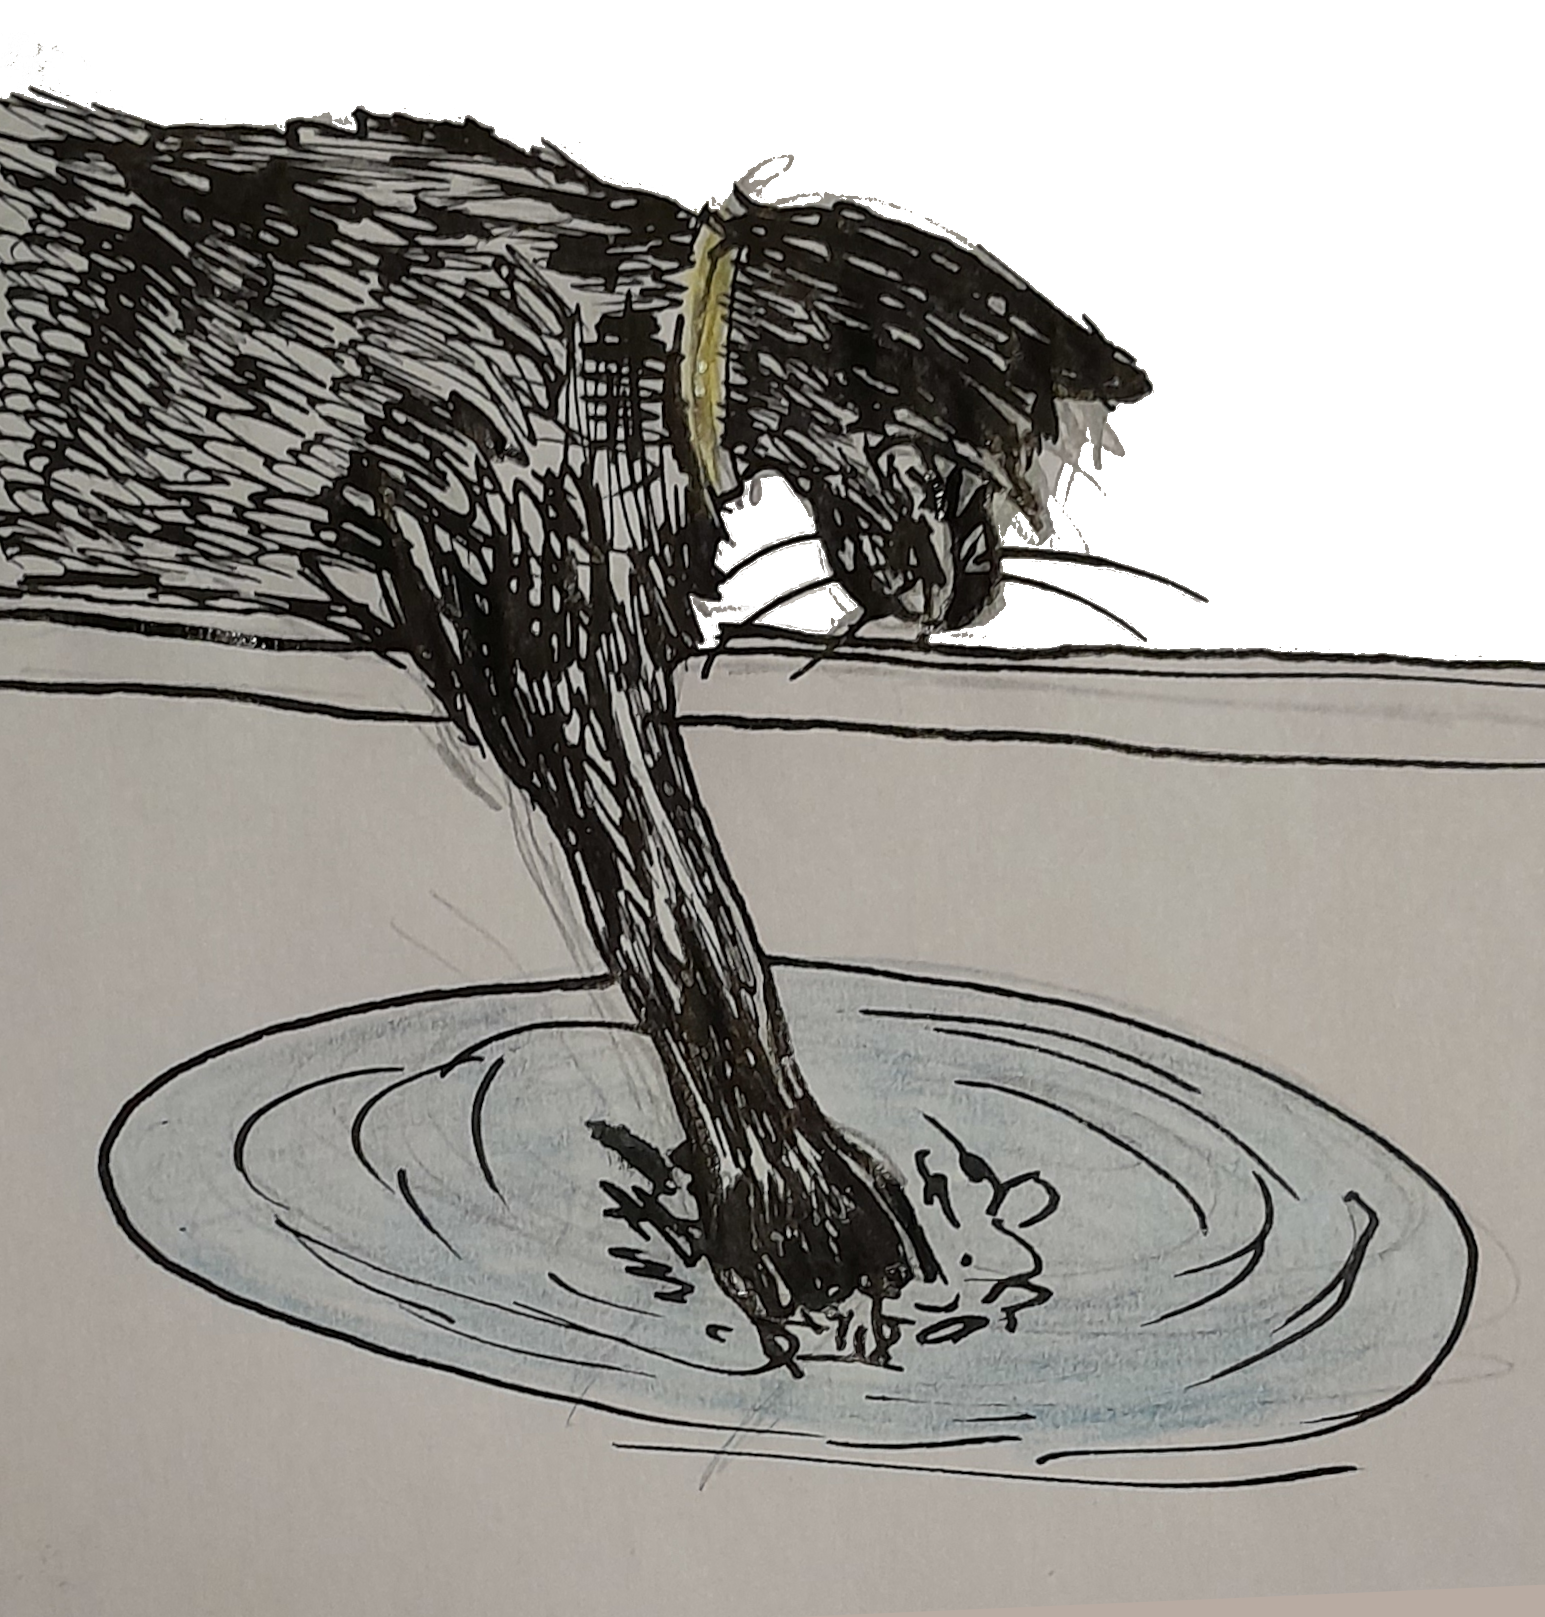
\includegraphics[width=\linewidth]{ottoko_vortex.png}};
	\end{tikzpicture}
\end{wrapfigure}
RECORDÉ LOS REMOLINOS QUE ME GUSTAN HACER EN CASA CUANDO SE JUNTA AGUA EN LA PILETA DE LA COCINA, O DONDE SEA. HAY QUE SER SUAVE CON EL AGUA, SI NO, NO SIGUE NUESTRO MOVIMIENTO Y SE DESARMA. CON PRECISIÓN FELINA CONSIGO QUE TODO SE MUEVA GIRANDO UNIFORME, SOBRE LA SUPERFICIE LIBRE DEL AGUA OBSERVABA ONDULACIONES QUE MANEJABA CON DESTREZA CON LAS GARRITAS DE MI PATA DELANTERA.

PENSABA QUE MIS PATAS NO ERAN DE LO MEJOR PARA MOVER AL AGUA. 

\newpage
\begin{tikzpicture}[remember picture, overlay]
	\node [inner sep=0pt, minimum width=\paperwidth, minimum height=\paperheight,opacity=.4] at (current page.center) {
\includegraphics[width=\paperwidth,height=\paperheight,angle=0]{paper31}};
\end{tikzpicture}

ALGUNA VEZ HABÍA PENSADO QUE SI MIS DEDOS ESTUVIERAN JUNTOS, UNIDOS POR ALGUNA MEMBRANA, EMPUJARÍAN MEJOR EL LÍQUIDO SIN TANTO BARULLO. Y VOLVÍ DE MIS PENSAMIENTOS A LA OBSERVACIÓN DE LOS TIBURONES.

PUDE DISTINGUIR SUS CINCO ALETAS. LA ALETA TRASERA O CAUDAL, QUE IMPULSA,SE MUEVE POR LOS FUERTES MÚSCULOS DE LA COLA.

\begin{center}

\begin{minipage}[r]{.7\textwidth}%\hspace{-2cm}
	\begin{tikzpicture}
		\node[xshift=1cm] () {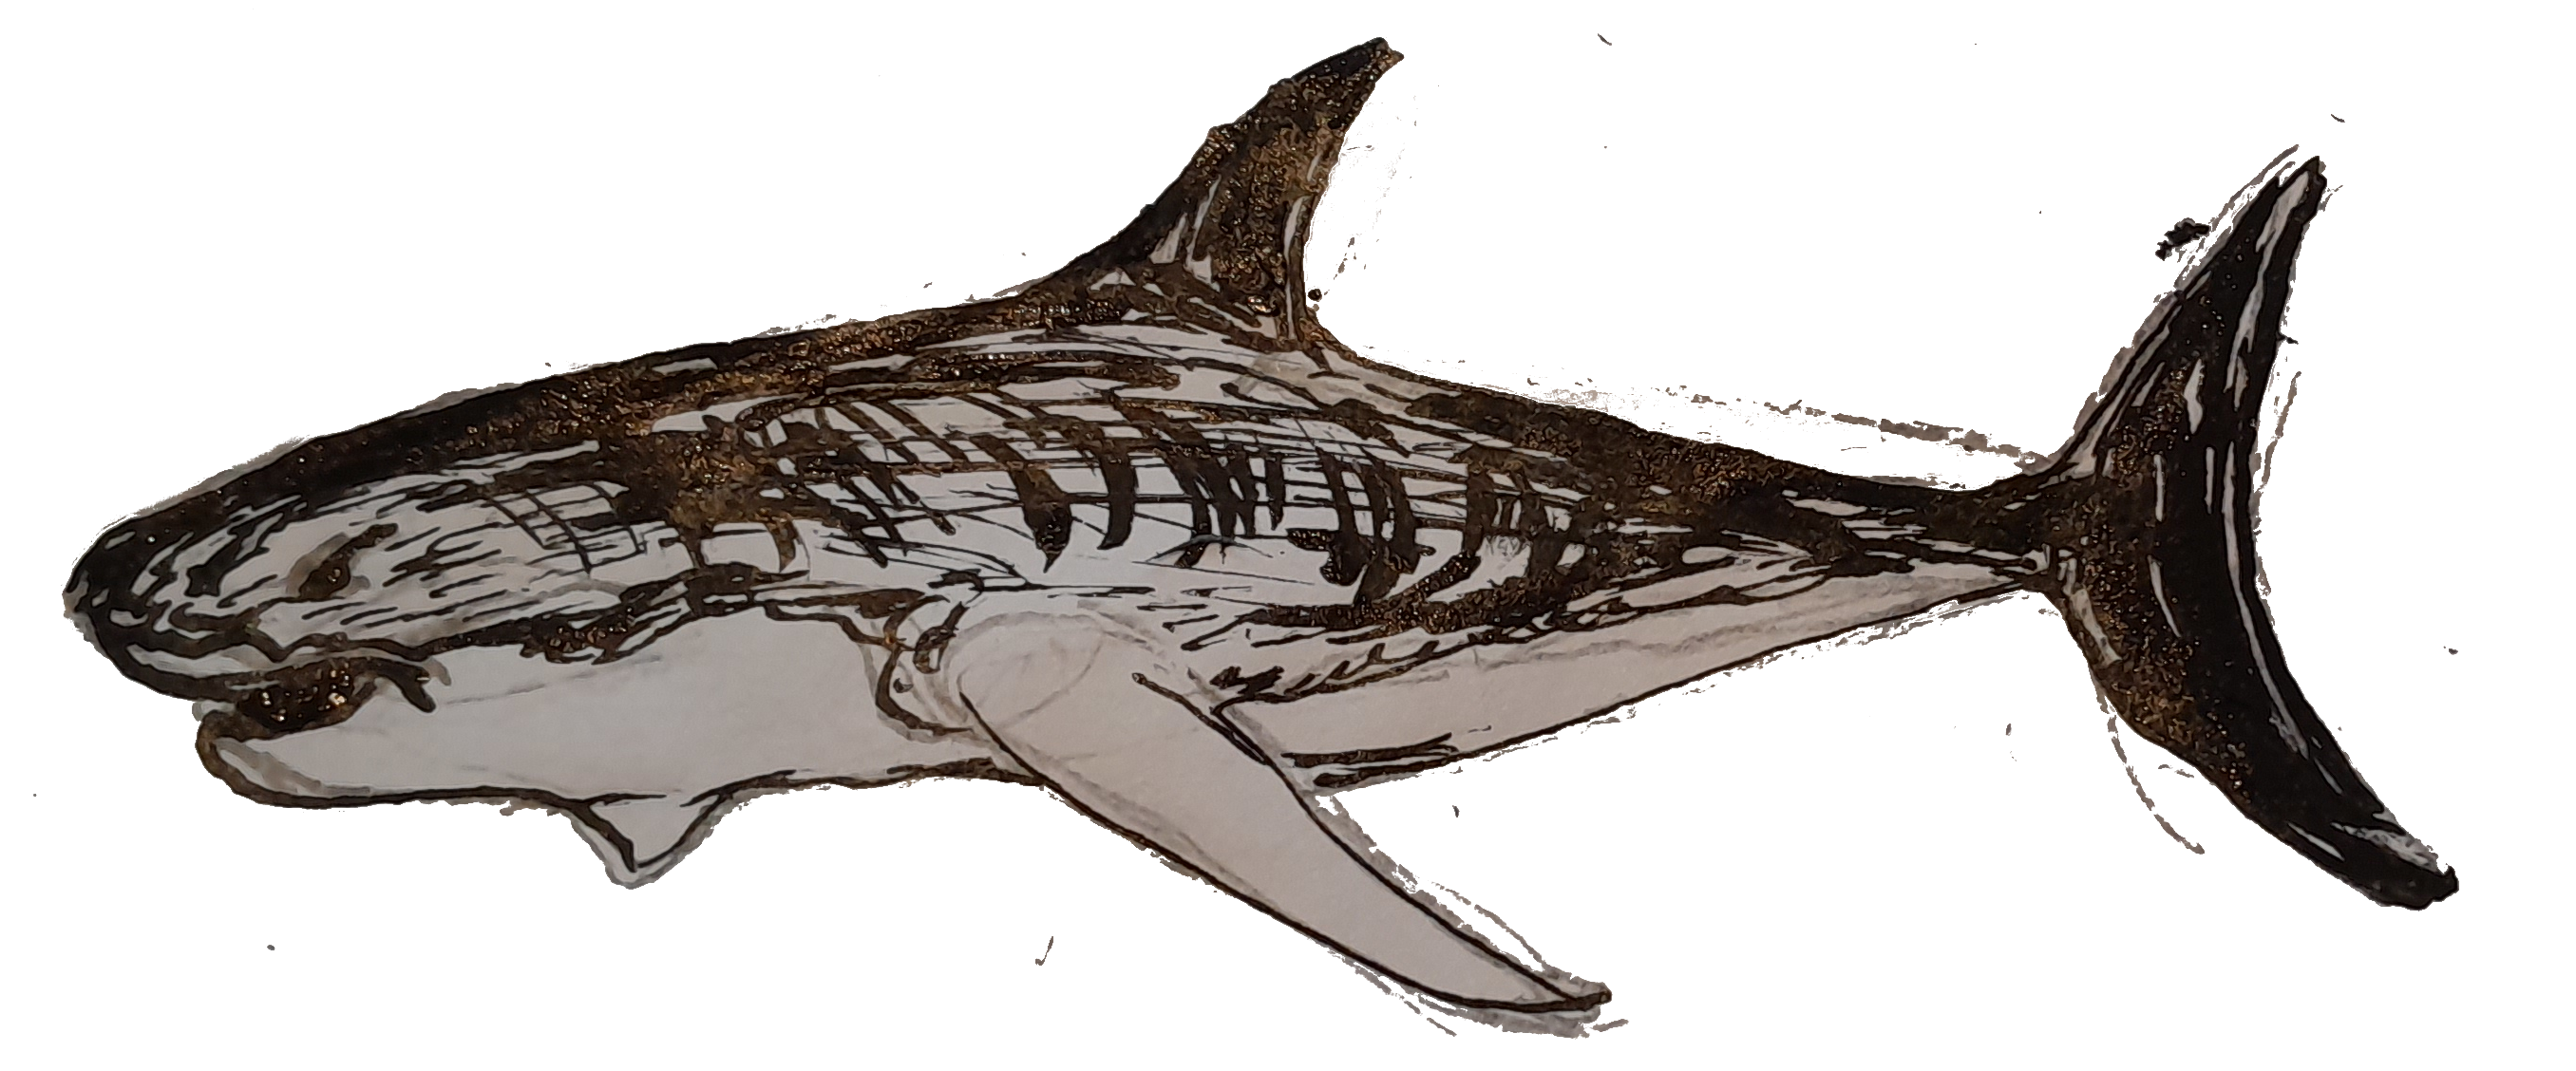
\includegraphics[width=\textwidth]{tiburon_perfil.png}};
	\end{tikzpicture}
\end{minipage}
	
\end{center}
\newpage
\begin{tikzpicture}[remember picture, overlay]
	\node [inner sep=0pt, minimum width=\paperwidth, minimum height=\paperheight,opacity=.4] at (current page.center) {
\includegraphics[width=\paperwidth,height=\paperheight,angle=0]{paper31}};
\end{tikzpicture}

 LA ALETA DORSAL, ESA QUE SIEMPRE VEMOS SALIR DEL AGUA EN LAS PELÍCULAS, SIRVE PARA SU EQUILIBRO Y BALANCEO. Y TAMBIÉN LAS DOS ALETAS PECTORALES, QUE SON LAS QUE PUEDEN USAR LOS PECES GIRAR Y TAMBIÉN PARA SU ESTABILIDAD. CUANDO NADAN, LAS REPLIEGAN SOBRE EL CUERPO PARA NO FRENARSE.
 
 SE PREGUNTARÁN COMO UN HUMILDE GATITO NEGRO HA PODIDO APRENDER ESTAS CUESTIONES, PUES LES DIRÉ QUE EN EL MUSEO, ADEMÁS DE LOS HUESOS, LOS BICHOS DISECADOS, LAS MAQUETAS, LOS ANIMALES EMBALSAMADOS, HAY MUCHÍSIMA GENTE QUE TRABAJA. PROFESORES, INVESTIGADORES, ESTUDIANTES, TÉCNICOS, ORDENANZAS, ADMINISTRADORES, PUES SÍ, MUCHA GENTE ALLÍ MISMO Y EN OTROS EDIFICIOS. Y HE PODIDO ESCUCHAR MÁS DE UNA INTERESANTE CHARLA AMPARADO POR LA LUZ TENUE.
 
 
 \newpage
 \begin{tikzpicture}[remember picture, overlay]
 	\node [inner sep=0pt, minimum width=\paperwidth, minimum height=\paperheight,opacity=.4] at (current page.center) {
\includegraphics[width=\paperwidth,height=\paperheight,angle=0]{paper29}};
 \end{tikzpicture}
MI PAPÁ ME CUENTA SOBRE LOS MUSEOS QUE, ADEMÁS DE TANTA CIENCIA Y TESOROS, NO HAY NADA MÁS PRECIOSO QUE EL RECUERDO DE USTEDES DISFRUTÁNDOLOS.
 
\begin{center}
	
	\begin{minipage}[r]{.7\textwidth}%\hspace{-2cm}
		\begin{tikzpicture}
			\node[xshift=1cm] () {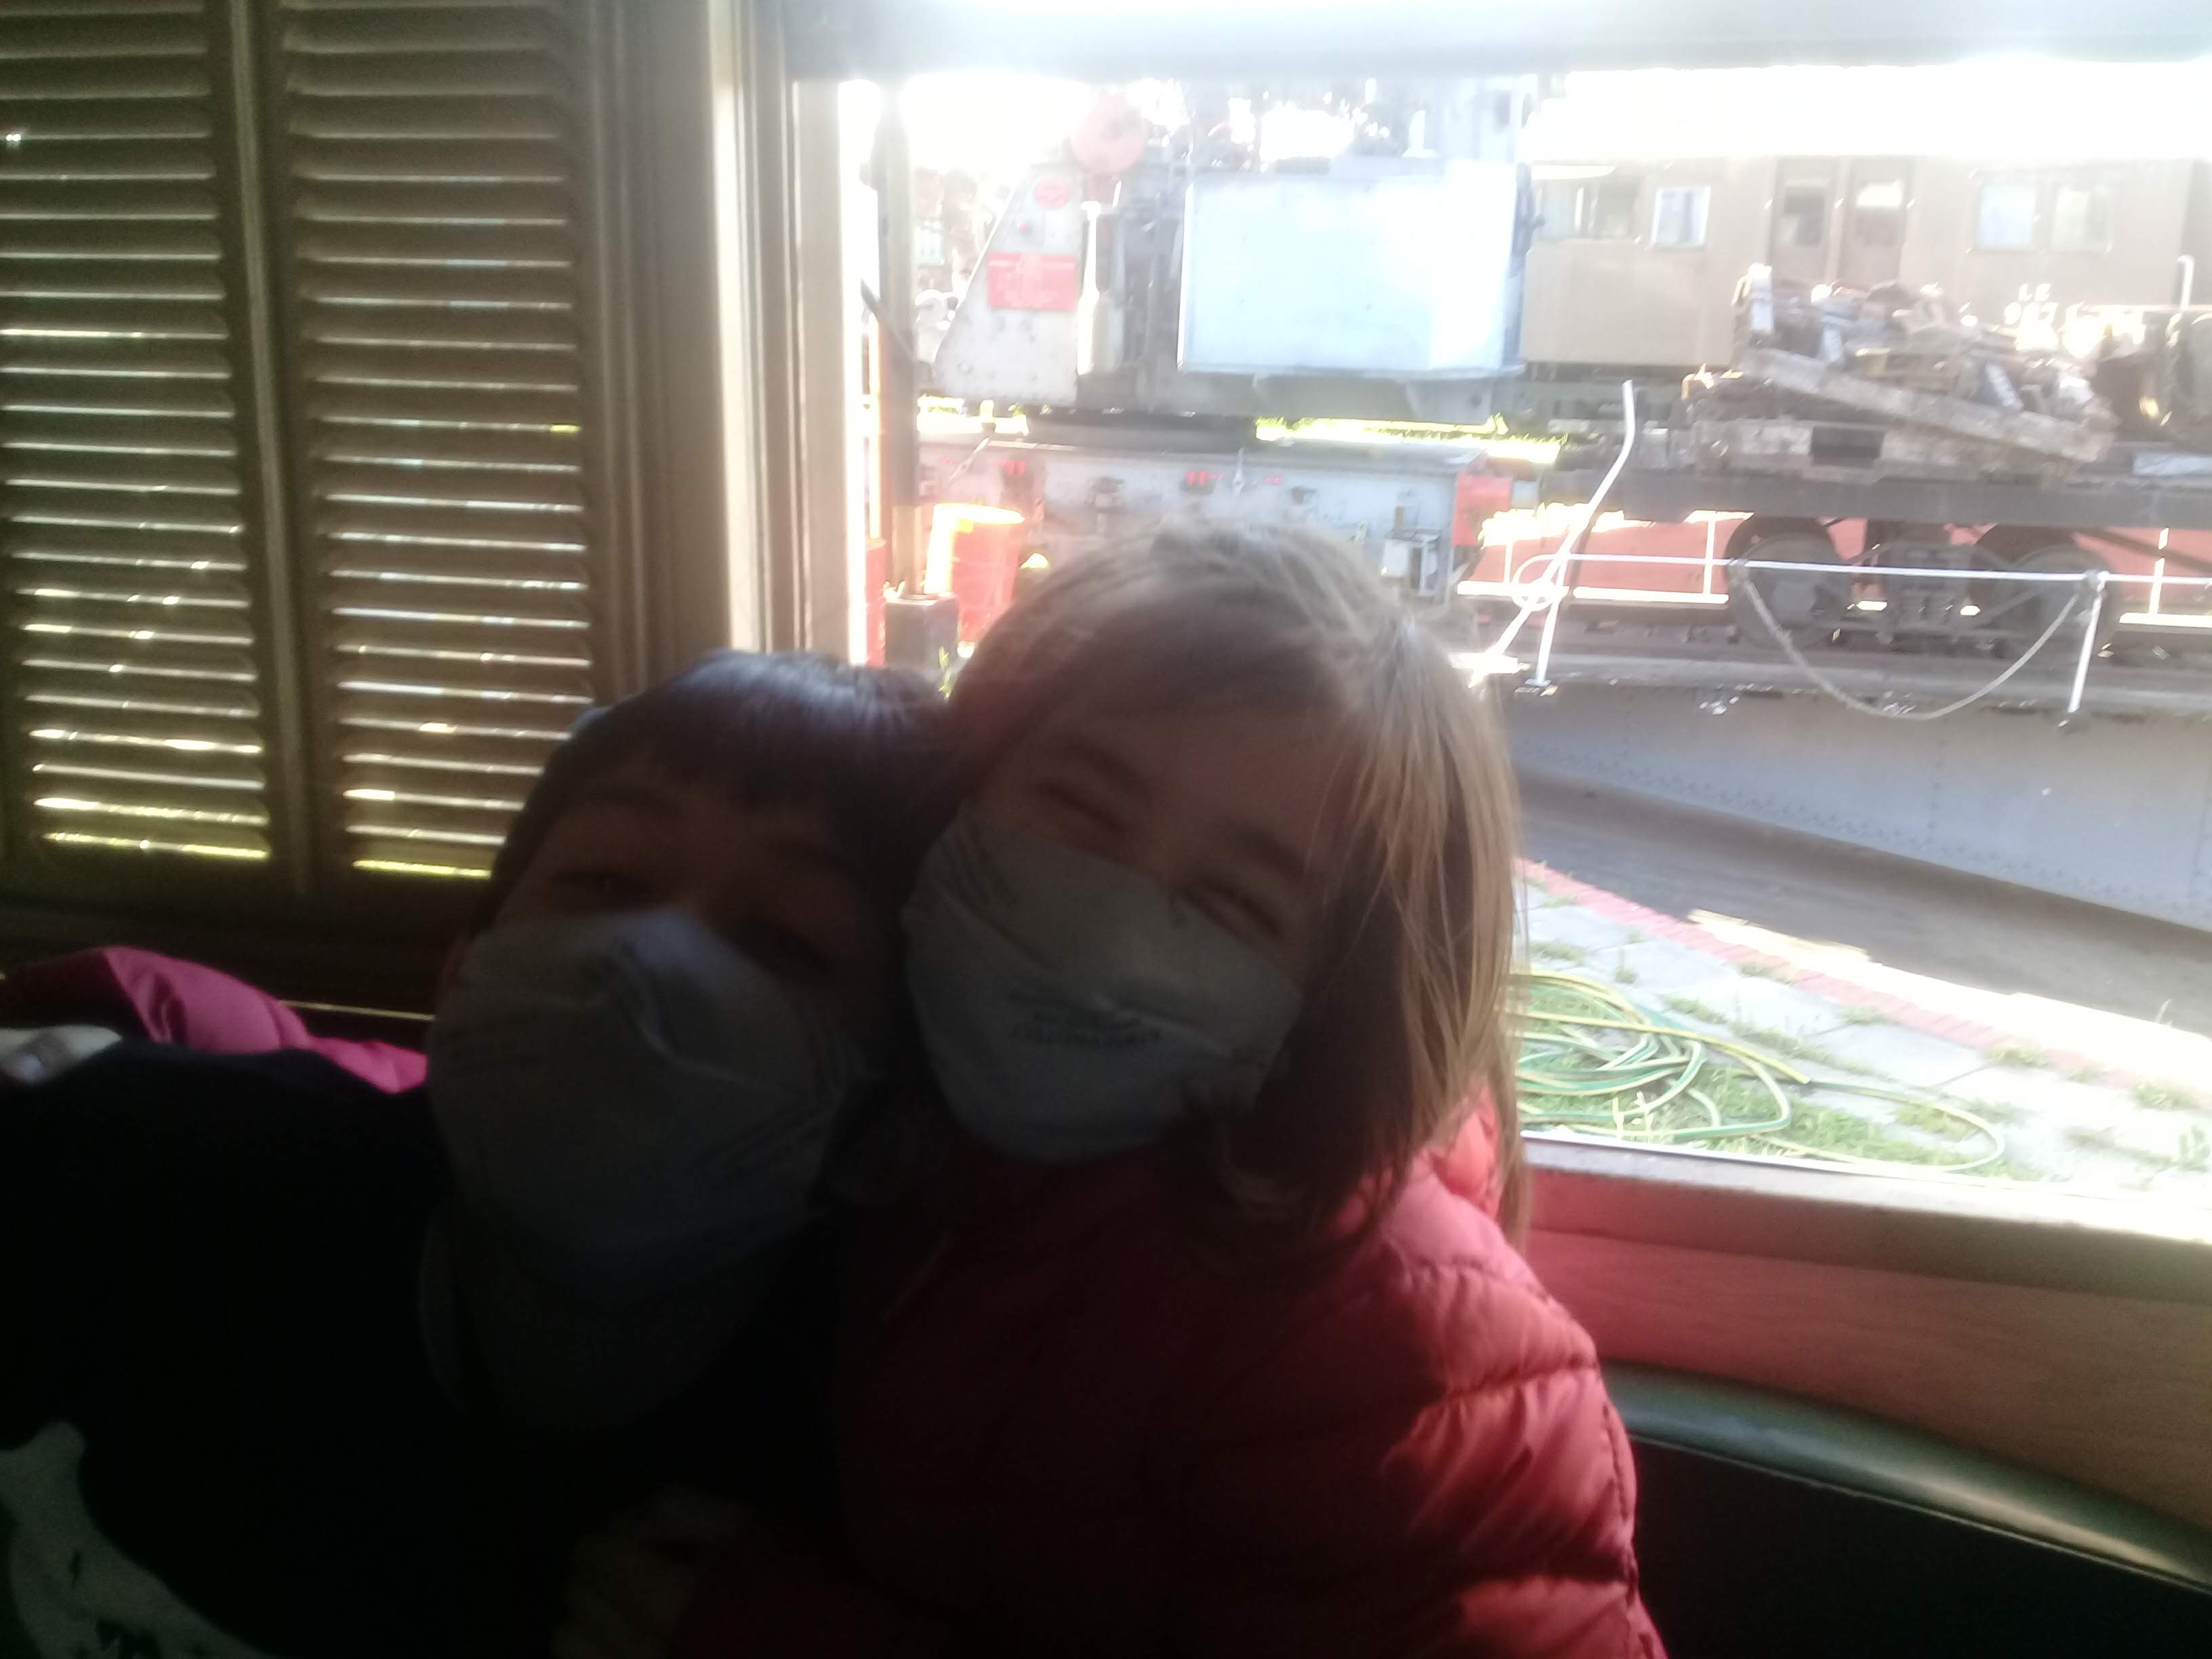
\includegraphics[width=\textwidth]{museo_lynch}};
		\end{tikzpicture}
	\end{minipage}
	
\end{center}


\newpage
\begin{tikzpicture}[remember picture, overlay]
	\node [inner sep=0pt, minimum width=\paperwidth, minimum height=\paperheight,opacity=.4] at (current page.center) {
\includegraphics[width=\paperwidth,height=\paperheight,angle=0]{paper31}};
\end{tikzpicture}

ALGUNOS ESTUDIOSOS DEBATÍAN SOBRE EL MOVIMIENTO DE LA ALETA DE LA COLA, SOBRE EL TAMAÑO, LA VELOCIDAD DE NADO DEL TIBURÓN Y EL MOVIMIENTO DEL AGUA AL DESPLAZARSE.

	\begin{minipage}[r]{.45\textwidth}%\hspace{-2cm}
		\begin{tikzpicture}
			\node[xshift=1cm] () {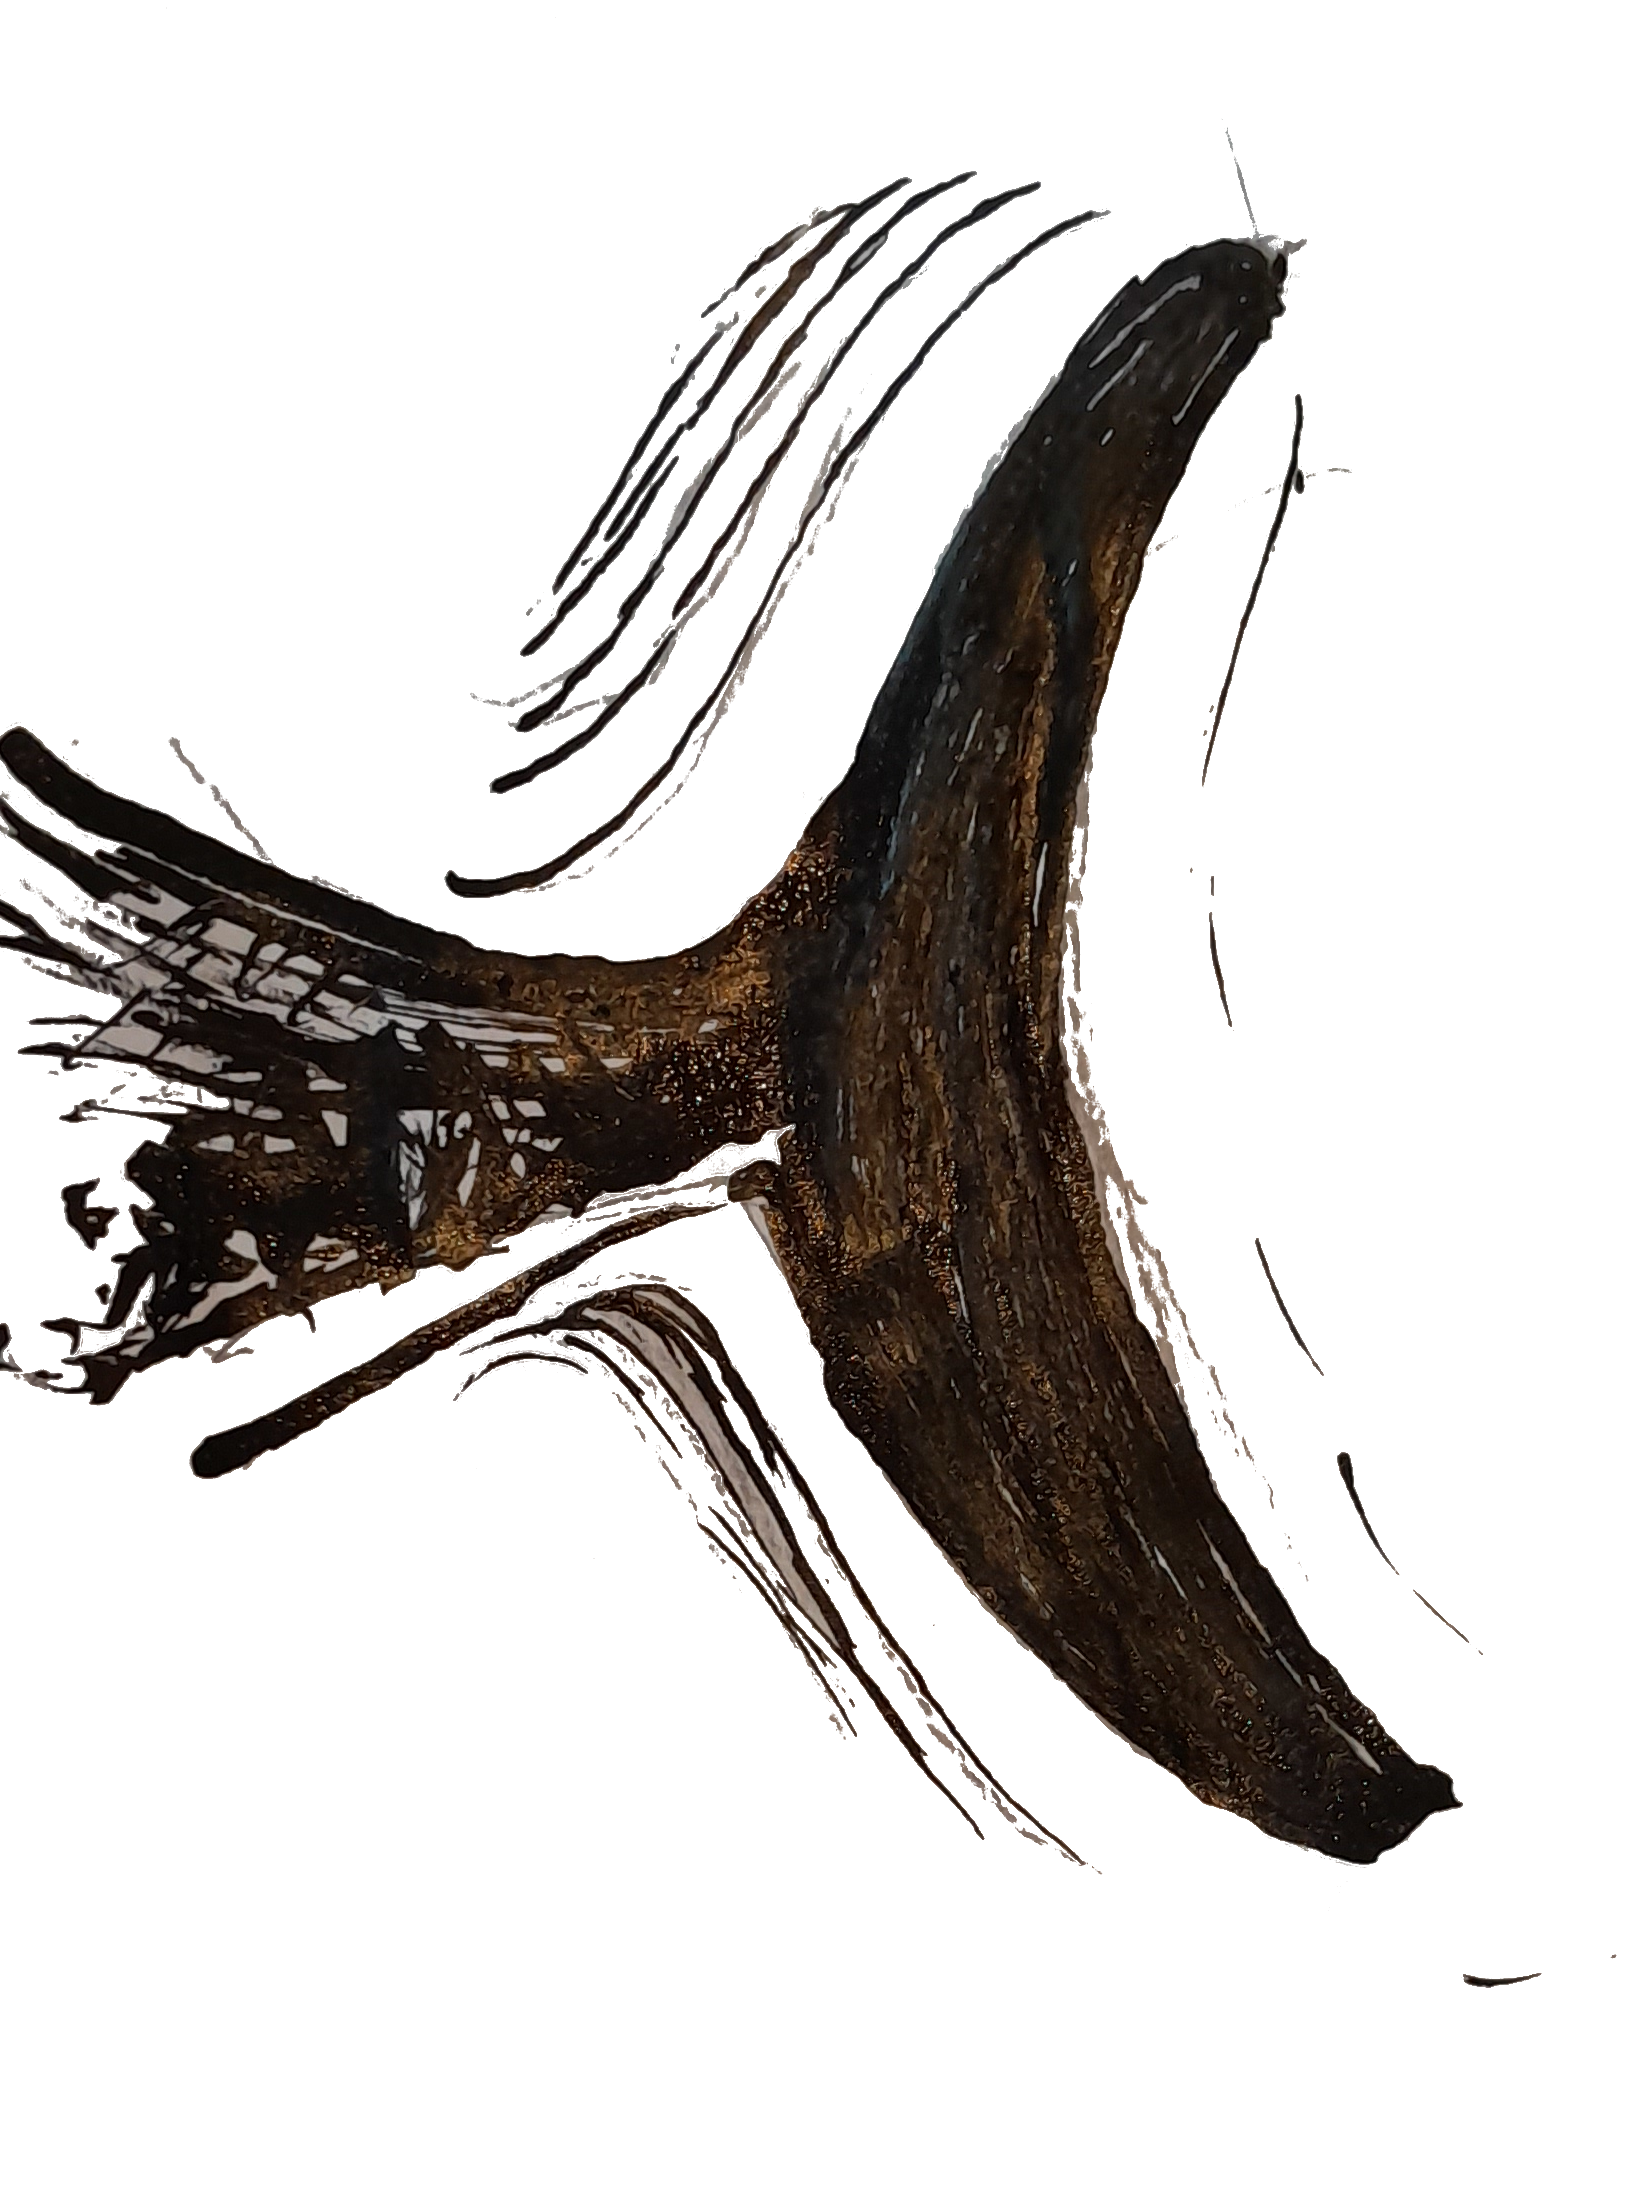
\includegraphics[width=.7\textwidth]{tiburon_aleta.png}};
		\end{tikzpicture}
	\end{minipage}\hfill
	\begin{minipage}[r]{.45\textwidth}%\hspace{-2cm}
	ALGUNAS DE ESTAS COSAS LAS HABÍA VISTO EN EL HERMOSO LIBRO DE JULES VERNE, VEINTE MIL LEGUAS DE VIAJE SUBMARINO. RECUERDO LAS TEORÍAS DE LOS PROFESORES DEL JARDIN DES PLANTES   SOBRE ENORMES CRIATURAS MARINAS.		
	\end{minipage}	

¿SE INTERESARÍAN TAMBIÉN POR FELINOS CURIOSOS?

\newpage
\begin{tikzpicture}[remember picture, overlay]
	\node [inner sep=0pt, minimum width=\paperwidth, minimum height=\paperheight,opacity=.4] at (current page.center) {
\includegraphics[width=\paperwidth,height=\paperheight,angle=0]{paper31}};
\end{tikzpicture}

\begin{minipage}[r]{.45\textwidth}%\hspace{-2cm}
	\begin{tikzpicture}
		\node[xshift=1cm] () {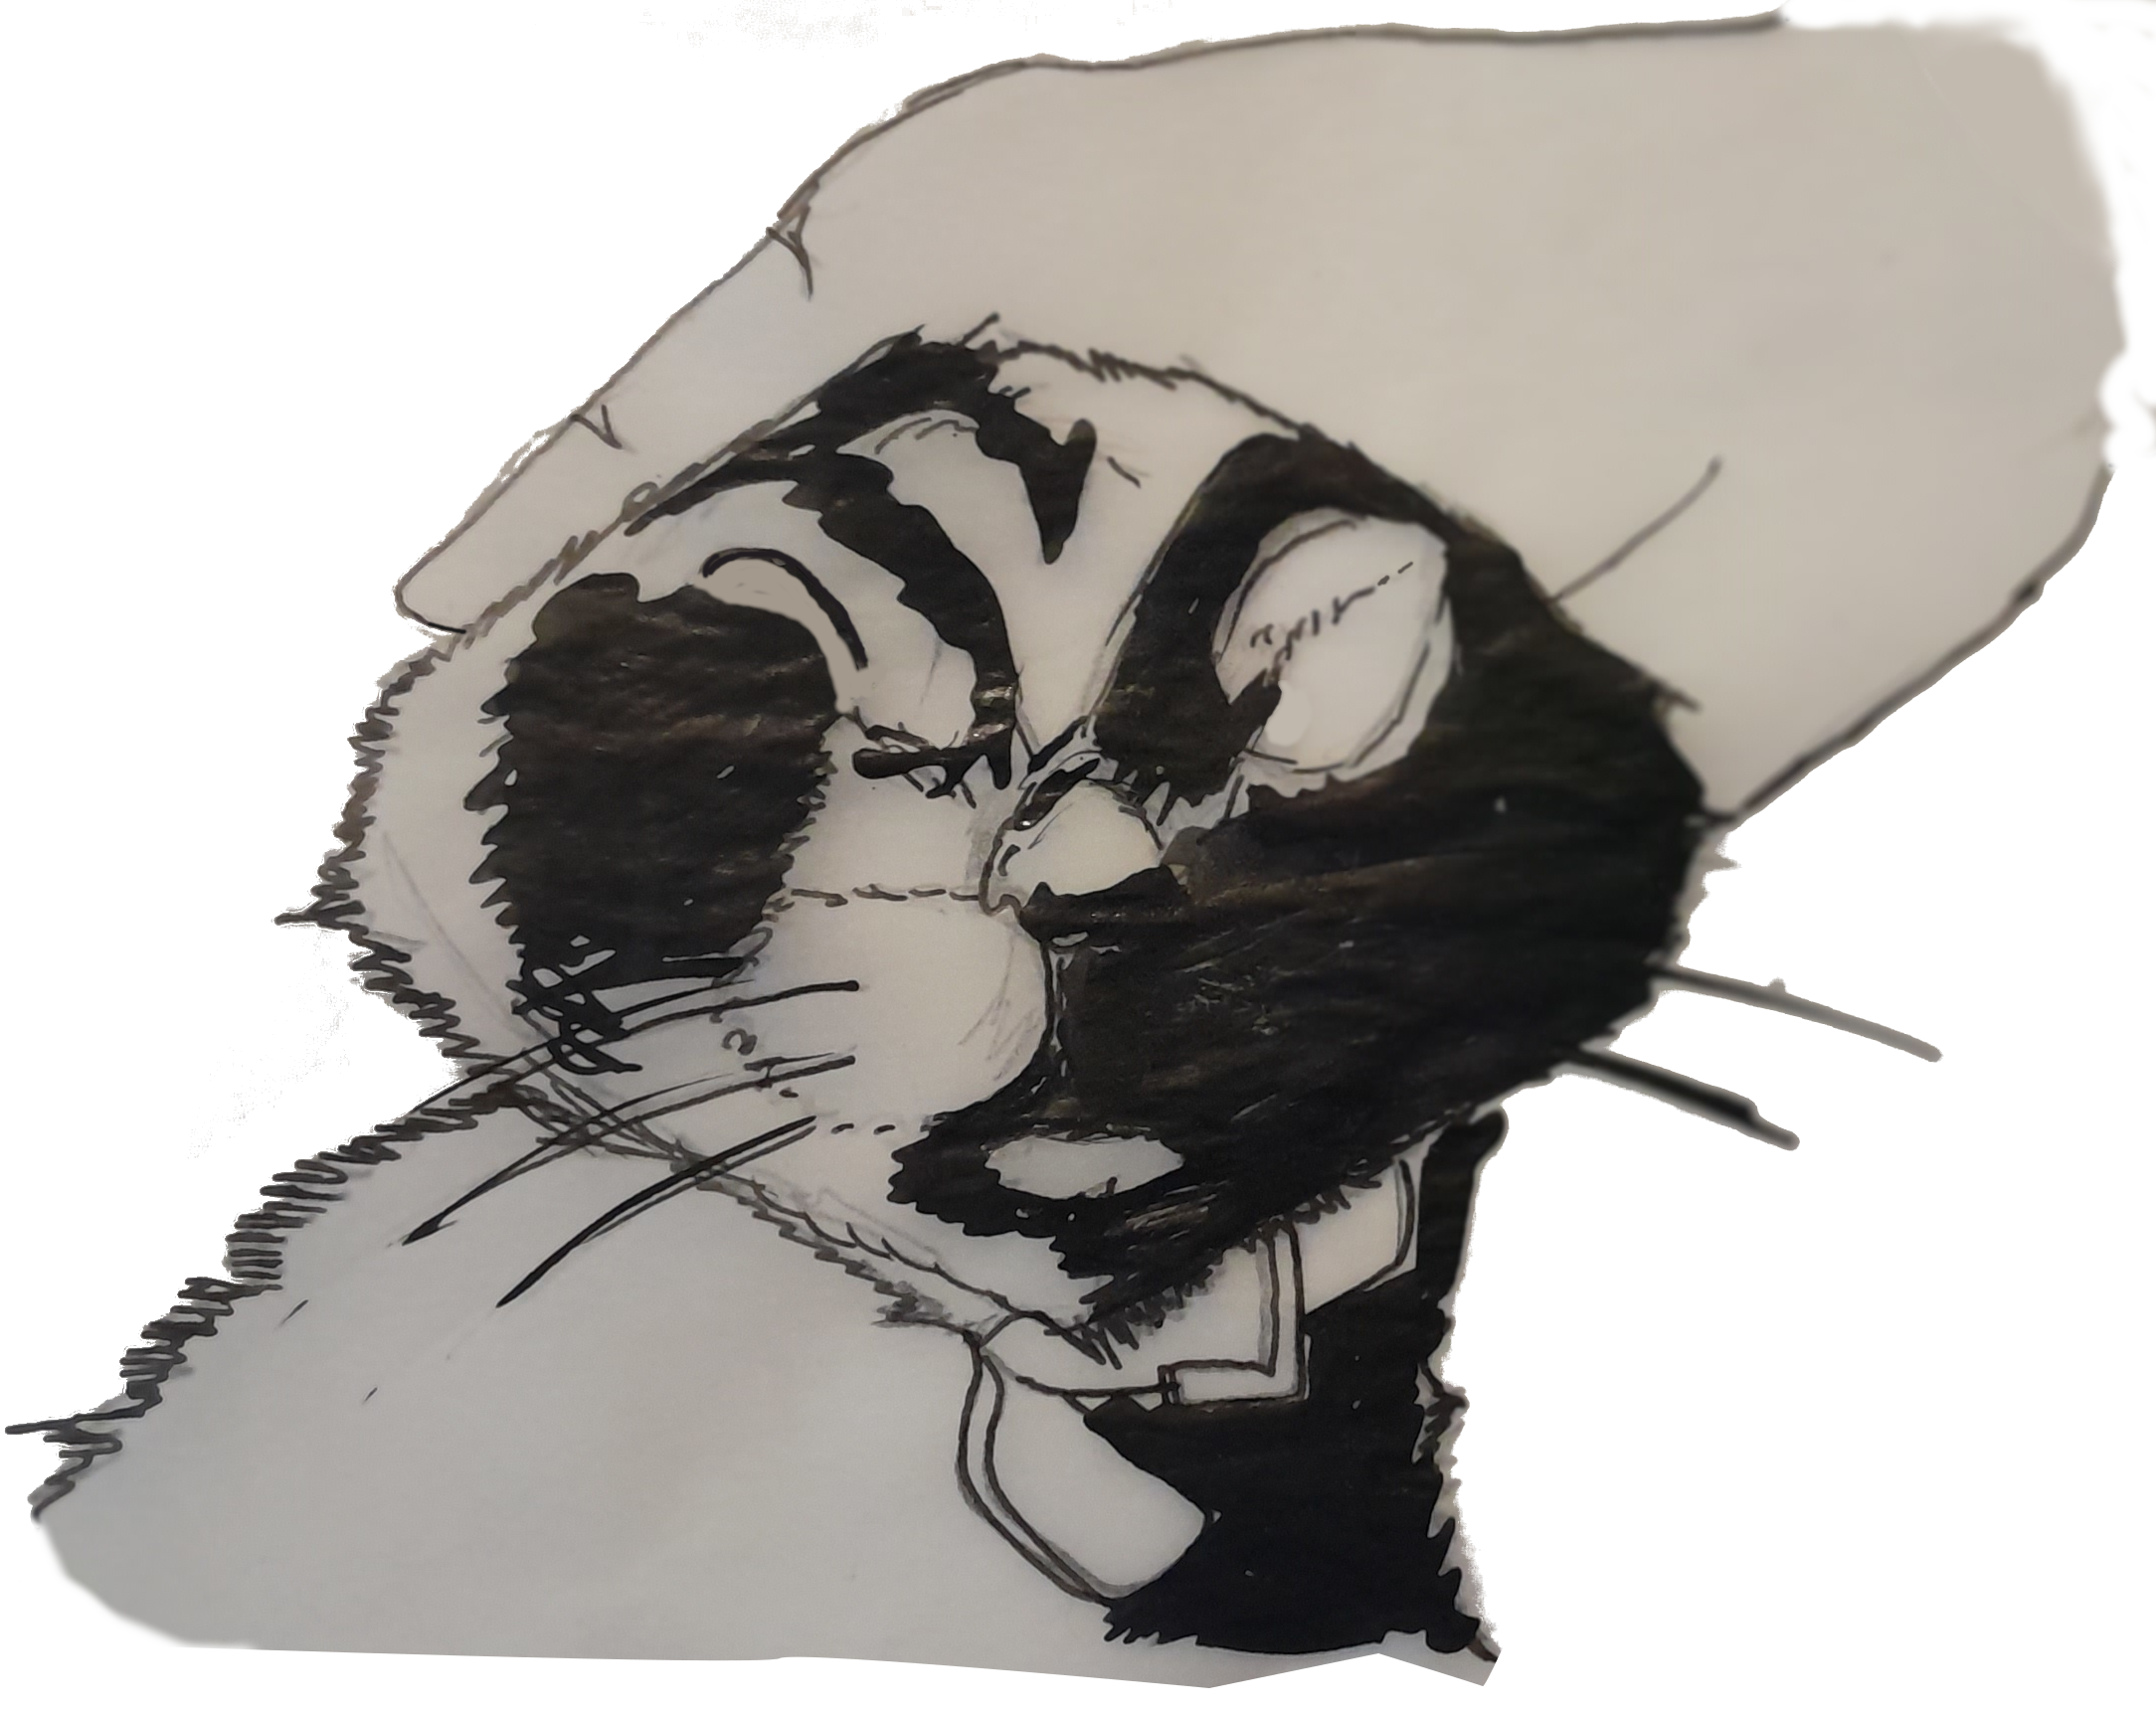
\includegraphics[width=\textwidth]{ottoko_plumin1.png}};
	\end{tikzpicture}
\end{minipage}\hfill
\begin{minipage}[r]{.45\textwidth}%\hspace{-2cm}
ADEMÁS DE SABIOS EN BIOLOGÍA, OBSERVÉ QUE HABÍA VARIOS AFICIONADOS AL DIBUJO Y A LA PINTURA. MÁS DE UNA VEZ VI JÓVENES ESTUDIANTES CON ANOTADORES, CUADERNOS, LÁPICES, MARCADORES Y PINTURITAS COPIANDO DESDE DISTINTOS ÁNGULOS A LOS ANIMALES DE CADA SALA.		
\end{minipage}	
\newpage
\begin{tikzpicture}[remember picture, overlay]
	\node [inner sep=0pt, minimum width=\paperwidth, minimum height=\paperheight,opacity=.4,color=Aquamarine4,fill=Aquamarine4!30!White] at (current page.center) {
\includegraphics[width=\paperwidth,height=\paperheight,angle=0,]{paper31}};
\end{tikzpicture}
\begin{center}
\begin{minipage}[r]{.7\textwidth}\hspace{-2cm}
	\begin{tikzpicture}
		\node[xshift=1cm] () {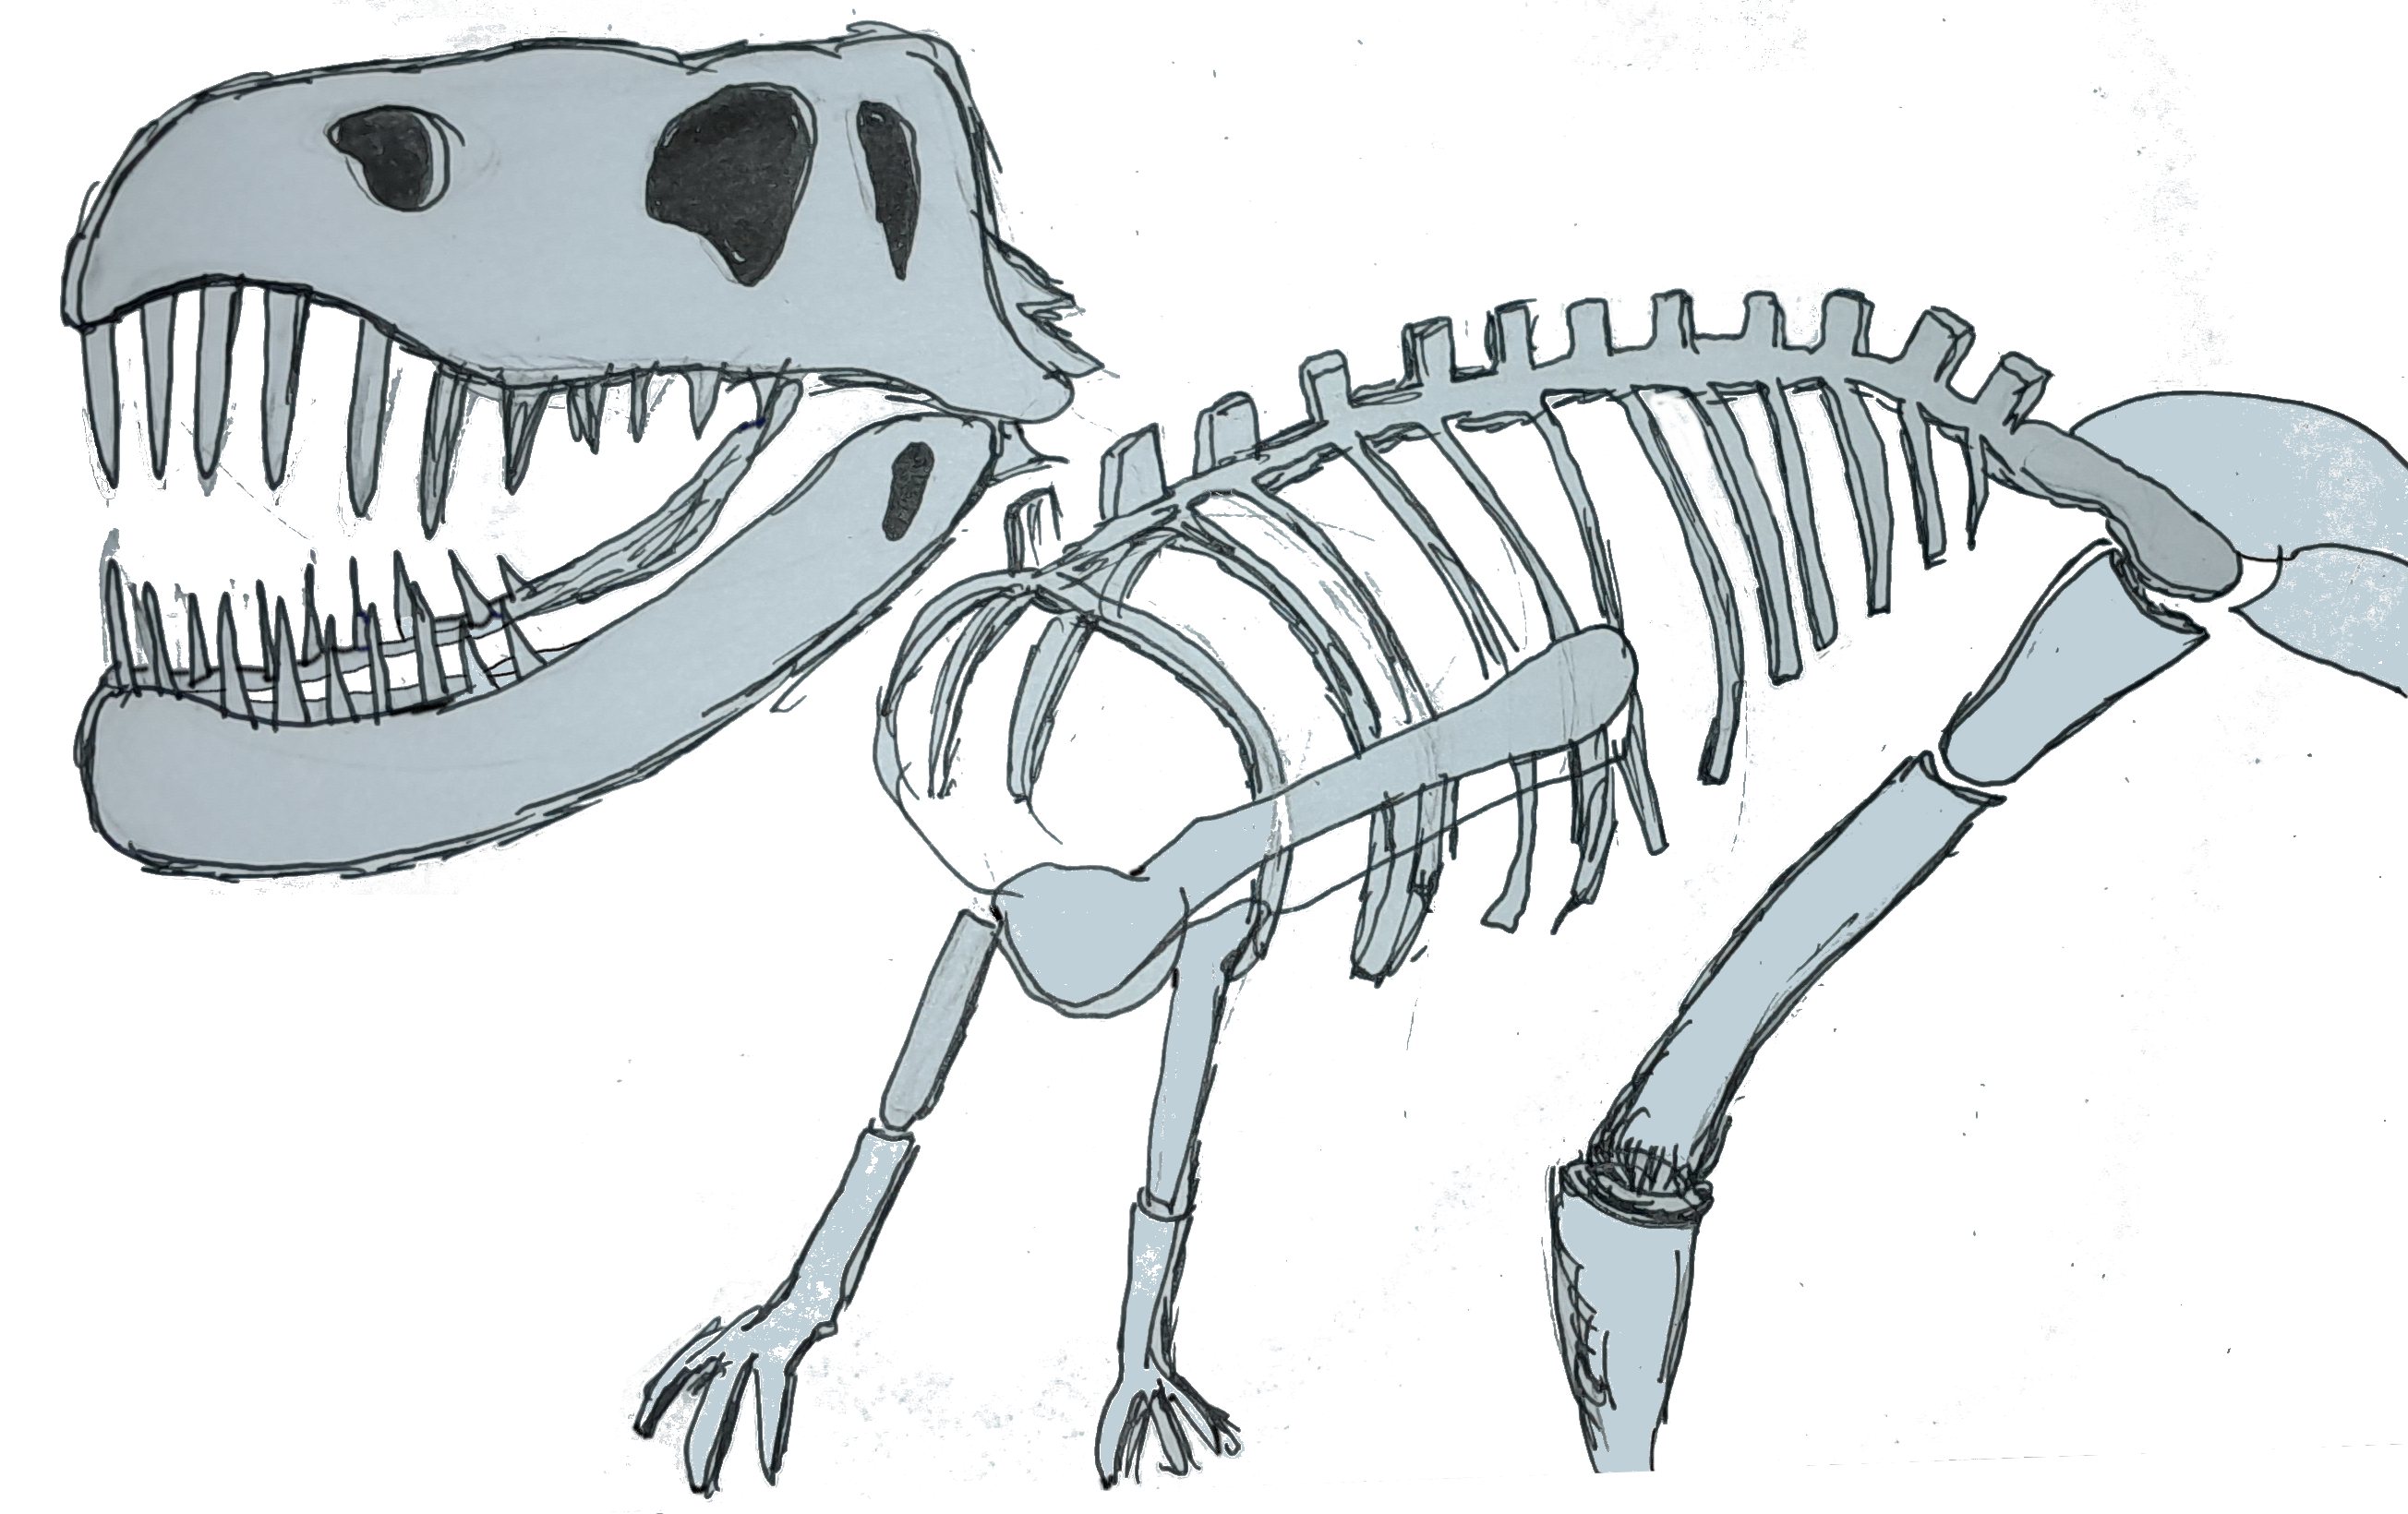
\includegraphics[width=\textwidth]{dino1.png}};
	\end{tikzpicture}
\end{minipage}	
\end{center}
FUE ENTONCES QUE INGRESÉ A UNA ENORME SALA QUE, EN UN PRINCIPIO, ME HIZO ARQUEAR TODO EL LARGO DE MI COLUMNA VERTEBRAL. 

\newpage
\begin{tikzpicture}[remember picture, overlay]
	\node [inner sep=0pt, minimum width=\paperwidth, minimum height=\paperheight,opacity=.4,color=Aquamarine4,fill=Aquamarine4!30!White] at (current page.center) {
\includegraphics[width=\paperwidth,height=\paperheight,angle=0,]{paper31}};
\end{tikzpicture}
PUES EN SU INTERIOR SE ENCONTRABAN INNUMERABLES BESTIAS GIGANTESCAS, LAGARTOS TERRIBLES DE PROPORCIONES DESMESURADAS. EL PRIMERO QUE VI TENÍA UNA QUIJADA GIGANTESCA, CASI DEL TAMAÑO DE UNA PERSONA, Y UN CUERPO NECESARIO PARA PODER SOSTENERLA, LAS PATAS TRASERAS PARECÍAN MUY POTENTES ASÍ COMO SU COLA, TODO FUERA PARA GUIAR A ESA ESPANTOSA Y DESCOMUNAL CABEZA DE DIENTES INTIMIDANTES COMO ESPADAS.

SE TRATABA DEL FAMOSO TYRANOSAURIO REX, MAGNÍFICO DEPREDADOR DE LA ERA DE LOS DINOSAURIOS. UN CAZADOR BIEN DISTINTO A NOSOTROS LOS FELINOS. PUES ERA PURA FUERZA BRUTA, EL ATAQUE DEBÍA SER UN DESPLIEGUE DIRECTO CONTRA GRANDES DINOSAURIOS HERVÍBOROS, PESADOS Y CON POCA CAPACIDAD DE REACCIÓN. PERO TAMBIÉN LEÍ QUE TENÍAN UNA VISIÓN PRIVILEGIADA, Y QUE DEBÍAN USARLA PARA CAZAR CON PRECISIÓN TAMBIÉN.

\newpage
\begin{tikzpicture}[remember picture, overlay]
	\node [inner sep=0pt, minimum width=\paperwidth, minimum height=\paperheight,opacity=.4,color=Aquamarine4,fill=Aquamarine4!30!White] at (current page.center) {
\includegraphics[width=\paperwidth,height=\paperheight,angle=0,]{paper31}};
\end{tikzpicture}

SI BIEN ME IMPRESIONARON PRIMERO LOS GIGANTESCOS T REX, DEBO DECIR QUE TODA LA COLECCIÓN DE DINOSAURIOS ES MAGNÍFICA EN EL MUSEO. A SU LADO SE DESTACABAN LOS SAURÓPODOS, LOS MÁS GRANDES DINOSAURIOS TERRESTRES. PARECE QUE NO ERAN LA PRESA PREFERIDA DE LOS TIRANOSAURIOS PUES MOVIÉNDOSE EN MANADA LOGRABAN DEFENDERSE USANDO SUS COLA GIGANTES COMO SI FUERAN LÁTIGOS. OTROS DEPREDADORES TEMIBLES ERAN LOS  VELOCIRAPTORS. AUNQUE DENTRO DE SU CLASE DE ANIMALES ERAN VELOCES COMO INDICA SU NOMBRE, ENTIENDO QUE NO PODRÍAN ALCANZAR A UN GATO, ¡AL MENOS POR UN BREVE MOMENTO! PERO CAZABAN EN GRUPO Y SERÍAN MUY PELIGROSOS SIN DUDAS.

EL HERRERASAURUS, DISPUESTO EN UN COSTADO, TENÍA UNA EXPRESIÓN NO MUY CALMA. 

\definecolor{celeste1}{HTML}{a7b7bf}
\newpage
\begin{tikzpicture}[remember picture, overlay]
	\node [inner sep=0pt, minimum width=\paperwidth, minimum height=\paperheight,opacity=1,color=Aquamarine4,fill=celeste1] at (current page.center) { };
\end{tikzpicture}



AUNQUE CONTABA CON DIENTES BASTANTE MÁS PEQUEÑOS, SERÍA UN PROBLEMA PARA LOS HERBÍVOROS DE LA ARGENTINA PREHISTÓRICA. 

\begin{wrapfigure} [7]{l}{.4\textwidth} 
	\begin{tikzpicture}
		\node[] () {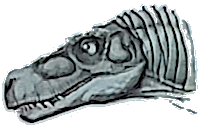
\includegraphics[width=.4\textwidth]{herrerasaurus1.png}};
	\end{tikzpicture}	
\end{wrapfigure}
	
O ESO FUE LO QUE PENSÉ, CUANDO ME DISTRAJE VIENDO COMO UNOS PEQUEÑOS SE ENTRETENÍAN EN UN GRAN ARENERO DISPUESTO AL LADO DE LOS HUESOS DE LOS FEROCES REPTILES. CON UN PINCEL Y SUS MANOS JUGABAN A DESCUBRIR FÓSILES Y A NO HACER PIS COMO SUPUSE EN UNA PRIMERA OJEADA. 

ASÍ DEBE HABER SIDO EL TRABAJO DE LOS PALEONTÓLOGOS Y DE TODOS AQUELLOS QUE HAN AYUDADO A DESCUBRIR TODOS ESOS FANTÁSTICOS HUESOS, COMO EL PASTOR VICTORINO HERRERA.

\newpage
\begin{tikzpicture}[remember picture, overlay]
	\node [inner sep=0pt, minimum width=\paperwidth, minimum height=\paperheight,opacity=1,color=Aquamarine4,fill=celeste1] at (current page.center) { };
\end{tikzpicture}
 SEGÚN LA HISTORIA, UN DESTACADO MIEMBRO DE LA UNIVERSIDAD DE TUCUMÁN, EL PROFESOR REIG, DIRIGIÓ LA EXPEDICIÓN Y DECIDIÓ LLAMAR AL DINOSAURIO CON EL NOMBRE DEL PASTOR. NO SÉ SI LO HIZO DE PURO GENEROSO O POR OTRAS RAZONES PERO ASÍ QUEDÓ.
 
 TODA LA SALA ES UNA VERDADERA MARAVILLA, ENTIENDO QUE PASEN TANTAS PERSONAS POR DÍA. Y QUE MUCHAS DE ELLAS VUELVAN Y VUELVAN SOBRE SUS PASOS. AÚN CONSIDERANDOME UNO DE LOS MÁS DESTACADOS DEPREDADORES DE NUESTRO MUNDO, NO PUEDO DEJAR DE SENTIR HUMILDAD A LADO DE TODOS ESOS GIGANTESCOS ANIMALES.
 
 LUEGO DE ATRAVESAR EL ESPACIO DEDICADO A LOS DINOSAURIOS, LLEGUÉ A UNA SALA DONDE SE VEÍAN MAMÍFEROS PREHISTÓRICOS. UNOS OSOS DE DESMESURADO TAMAÑO LLAMADOS ARCTOTHERIUMS. TAMBIÉN MAMUTS, MASTODONTES Y MEGATERIOS.
 
  

